% This is samplepaper.tex, a sample chapter demonstrating the
% LLNCS macro package for Springer Computer Science proceedings;
% Version 2.20 of 2017/10/04
%
\documentclass[runningheads]{fmcad}
%
\usepackage{graphicx}
\usepackage{listings}
\usepackage[dvipsnames]{xcolor}
\usepackage{amsmath}
\usepackage[english]{babel}
\usepackage[misc]{ifsym}
\usepackage{subfloat}
\usepackage{float}
\usepackage{algorithmic} 
\usepackage{amssymb}
\usepackage{amsthm}
% \usepackage[colorlinks]{hyperref}
 
\newif\ifbadgeavailable\newif\ifbadgefunctional\newif\ifbadgereusable
\badgeavailabletrue\badgefunctionaltrue\badgereusablefalse
\usepackage{graphicx}
%\usepackage[firstpageonly=true,angle=0,vpos=.147\paperheight,hpos=.393\linewidth,vanchor=t,hanchor=l]{draftwatermark}

% \usepackage[beamer, customcolors]{hf-tikz}
\usepackage{blkarray}
\usepackage{tikz}

\usetikzlibrary{external}
% \tikzexternalize[prefix=Figures/]
\usepackage[normalem]{ulem}
\usepackage[ruled,linesnumbered,noend]{algorithm2e}
\usepackage{amsmath}
\usepackage[inline]{enumitem}
% \usepackage[colorlinks=false]{hyperref}
\definecolor{codegreen}{rgb}{0,0.6,0}
\definecolor{codegray}{rgb}{0.5,0.5,0.5}
\definecolor{codepurple}{rgb}{0.58,0,0.82}
\definecolor{backcolour}{rgb}{0.95,0.95,0.92}


\lstdefinestyle{mystyle}{
    backgroundcolor=\color{backcolour},
    commentstyle=\color{codegreen},
    keywordstyle=\color{magenta},
    numberstyle=\tiny\color{codegray},
    stringstyle=\color{codepurple},
    basicstyle=\ttfamily\footnotesize,
    breakatwhitespace=false,
    breaklines=true,
    captionpos=b,
    keepspaces=true,
    numbers=left,
    numbersep=5pt,
    showspaces=false,
    showstringspaces=false,
    showtabs=false,
    tabsize=2
}

\lstset{style=mystyle}
% Used for displaying a sample figure. If possible, figure files should
% be included in EPS format.
%
% If you use the hyperref package, please uncomment the following line
% to display URLs in blue roman font according to Springer's eBook style:
% \renewcommand\UrlFont{\color{blue}\rmfamily}

\usetikzlibrary{shapes, tikzmark, arrows, calc, positioning, intersections, automata, fit}
\usetikzlibrary{decorations.pathreplacing, arrows.meta}
\usetikzlibrary{decorations.pathmorphing}

% \newtheoremstyle{mydef}
% % {\topsep}{\topsep}%
% % {}{}%
% % {\bfseries}{}
% % {\newline}
% {%
% %   \rule{0.49\textwidth}{0.4pt}\\*%
%   \thmname{#1} \thmnote{.\ #2}.\\*[-1.5ex]%
% %   \rule{0.49\textwidth}{0.4pt}
% }%

% \theoremstyle{mydef}
\newtheorem{lemma}{Lemma}
\theoremstyle{definition}
\newtheorem{definition}{Definition}

\newtheorem{example}{Example}



\begin{document}

% \SetWatermarkText{%
% \raisebox{-4cm}% AUTHORS: Move the badge up/down; should be next to title, authors, or affiliations
% {\ifbadgeavailable\includegraphics[width=11mm]{Figures/FM_2024_AE_available}\hspace{.815\linewidth}\else\hspace{.905\linewidth}\fi%
% \ifbadgefunctional\includegraphics[width=11mm]{Figures/FM_2024_AE_functional}\fi}}

% TODO: Title to Multiloop analysis
% \title{TPA-enabled reachability analysis for multiloop programs}
% \title{Incremental loop-summarization based reachability analysis of software}
% \title{Incremental property-based cycle summarization for Constrained Horn Clauses solving of complex systems}
% \title{Summarization-Based Reachability Analysis via Constrained Horn Clauses}
\title{Safety-based Termination Analysis With Transition Invariant Generation}

% \titlerunning{Safety-based Termination Analysis With Transition Invariant Generation}
%
% \titlerunning{Reachability Analysis for Multiloop Programs Using TPA}
% If the paper title is too long for the running head, you can set
% an abbreviated paper title here
%
% \author{Konstantin Britikov(\Letter)\inst{1}
%  \orcidID{0009-0005-7843-7290}
% \and
% Natasha Sharygina\inst{1}
%  \orcidID{0000-0002-8872-4913}
% \and
% Grigory Fedyukovich\inst{1,2}
%  \orcidID{0000-0003-1727-4043}
% \and
% Martin Blicha\inst{1}
%  \orcidID{0000-0001-8140-4098}
% }


\author{Konstantin Britikov
% \inst{1}(\Letter)
%  \orcidID{0009-0005-7843-7290}
% \and
\and Martin Blicha
% \orcidID{0000-0003-1727-4043}
\and Grigory Fedyukovich
% \inst{2}
%  \orcidID{0000-0001-8140-4098}
\and Natasha Sharygina
% \inst{1}
%  \orcidID{0000-0002-8872-4913}
}
% \institute{}
% \authorrunning{Britikov K., Blicha M., Fedyukovich G., Sharygina N.}
% First names are abbreviated in the running head.
% If there are more than two authors, 'et al.' is used.
%
% \institute{University of Lugano, Lugano, Switzerland \and
% Florida State University, Tallahassee, FL, United States
% \email{lncs@springer.com}\\
 % \url{http://www.springer.com/gp/computer-science/lncs}

%
\maketitle              % typeset the header of the contribution
%


\begin{abstract}
    Termination analysis is difficult.
\end{abstract}

%



% \newcommand{\oreach}[1]{\ensuremath{\mathit{TPA}^{{\leq}#1}}}
% \newcommand{\oreachfull}[3]{\ensuremath{\oreach{#1}(#2,#3)}}
% \newcommand{\atrleq}[1]{\ensuremath{\mathit{TPA}^{{\leq}#1}}}
% \newcommand{\atreq}[1]{\ensuremath{\mathit{TPA}^{{=}#1}}}
% \newcommand{\atrlt}[1]{\ensuremath{\mathit{TPA}^{{<}#1}}}


% \newcommand{\trleq}[1]{\ensuremath{\mathit{R}^{{\leq}#1}}}
% \newcommand{\treq}[1]{\ensuremath{\mathit{R}^{{=}#1}}}
% \newcommand{\trlt}[1]{\ensuremath{\mathit{R}^{{<}#1}}}

% PRELIMINARIES  VARIABLES
\newcommand{\source}{\mathit{src}}
\newcommand{\target}{\mathit{trg}}
\newcommand{\constraint}{\mathit{constr}}
\newcommand{\clause}{\mathit{c}}
\newcommand{\clauses}{C}
\newcommand{\pred}{\mathit{p}}
\newcommand{\preds}{\mathcal{P}}
\newcommand{\predsf}{\mathit{preds}}
\newcommand{\system}{\mathit{S}}
\newcommand{\encoding}{\pi}
\newcommand{\node}{n}
\newcommand{\init}{\mathit{Source}}
\newcommand{\route}{{{{h}}}}
\newcommand{\routes}{\mathit{H}}
\newcommand{\iteration}{{{\gamma}}}
\newcommand{\proute}{{{\eta}}}
\newcommand{\proutes}{\Theta}
\newcommand{\query}{\mathit{Target}}
\newcommand{\incoming}{\mathit{\alpha}}
\newcommand{\outgoing}{\mathit{\omega}}
\newcommand{\vars}{\mathcal{V}}
\newcommand{\tr}{\mathit{Tr}}
\newcommand{\inv}{\mathit{Inv}}
\newcommand{\trInv}{\mathit{TrInv}}
\newcommand{\mop}{\mathit{MOP}}
\newcommand{\tpa}{\textsc{TPA}\xspace}
\newcommand{\res}{\mathit{res}}
\newcommand{\flas}{\mathit{Flas}}
\newcommand{\id}{\mathit{Id}}
\newcommand{\bad}{\mathit{Bad}}
\newcommand{\varsx}{\ensuremath{\vec{x}}}

\newcommand{\tuple}[1]{\langle #1 \rangle}

\newcommand{\unrollings}{\mathcal{U}}
\newcommand{\summaries}{\ensuremath{\Sigma}}
\newcommand{\summary}{\ensuremath{\sigma}}
% \newcommand{\inv}{\ensuremath{\inv}}
% \newcommand{\program}{\ensuremath{\mathcal{P}}}
% \newcommand{\cutpoints}{\ensuremath{\mathcal{CP}}}

% \newcommand{\predicates}{\mathcal{Ps}}



\newcommand{\false}{\mathit{false}}
\newcommand{\true}{\mathit{true}}


\newcommand{\SAFE}{\mathcal{SAFE}}
\newcommand{\UNSAFE}{\mathcal{UNSAFE}}
\newcommand{\DAG}{D}
\newcommand{\curr}{\mathit{curr}}




\newcommand{\gri}[1]{$[$\textbf{\textcolor{BrickRed}{Grigory}}:~~\emph{\textcolor{Mahogany}{#1}}$]$}
\newcommand{\martin}[1]{$[$\textbf{\textcolor{BrickRed}{Martin}}:~~\emph{\textcolor{blue}{#1}}$]$}
\newcommand{\konst}[1]{$[$\textbf{\textcolor{ForestGreen}{Konstantin}}:~~\emph{\textcolor{blue}{#1}}$]$}



% ALGORITHM



\newcommand{\cexp}{\ensuremath{\mathit{cexp}}}


\newcommand{\analyze}{\textsc{Analyze}\xspace}
\newcommand{\blockTerm}{\textsc{BlockTerm}\xspace}
% \newcommand{\extractPaths}{\textsc{ExtractPaths}\xspace}
% \newcommand{\queryUnrolling}{\textsc{ExpandPath}\xspace}
% \newcommand{\summarize}{\textsc{AnalyzeCycles}\xspace}

\newcommand{\inc}[1]{\ensuremath{{#1}^{\mathit{pre}}}}
\newcommand{\out}[1]{\ensuremath{{#1}^{\mathit{post}}}}
\newcommand{\checked}{\mathit{curr}}
\newcommand{\safe}[1]{\ensuremath{#1.\mathit{sat}}}
\newcommand{\mbp}{\ensuremath{\mathit{MBP}}\xspace}
\newcommand{\splittpa}{\textsc{TPA}}
\newcommand{\reached}{\ensuremath{\mathit{visited}}}
\newcommand{\blocked}{\ensuremath{\mathit{blocked}}}
\newcommand{\current}{\ensuremath{\mathit{curr}}}
\newcommand{\outp}{\ensuremath{\mathit{output}}}
\newcommand{\cex}{\ensuremath{\mathit{cex}}}
\newcommand{\iter}{\ensuremath{\mathit{depth}}}
\newcommand{\iterConst}{\ensuremath{\mathit{iterConst}}}
\newcommand{\iterReached}{\ensuremath{\mathit{iterVisited}}}
% \newcommand{\expansion}{\ensuremath{\mathit{exp}}}
\newcommand{\ex}{\ensuremath{\mathit{e}}}

\newcommand{\pop}{\ensuremath{\mathit{pop}}}
\newcommand{\learnedConst}{\mathit{constr}}
\newcommand{\precond}{\mathit{pre}}
\newcommand{\postcond}{\mathit{post}}
\newcommand{\sourcepred}{\mathit{s}}
\newcommand{\targetpred}{\mathit{t}}
% \newcommand{\id}{\mathit{Id}}



\newcommand{\model}{M}
\newcommand{\algorithmicbreak}{\textbf{break}}


\newcommand{\sat}{\textsc{SAT}}
\newcommand{\unsat}{\textsc{UNSAT}}



%

% \section{Introduction}
\label{Sec:Introduction}

Termination analysis of infinite-state systems is a fundamental problem 
in formal methods.
Proving termination and nontermination over LIA is generally undecidable~\cite{DBLP:conf/cav/Braverman06}, 
yet many practical techniques succeed on large classes of real-world 
programs.

Modern techniques treat termination and nontermination as separate 
problems, since each has a different proof procedure.
State-of-the-art termination techniques centre around the synthesis of 
ranking functions for the transition relation~\cite{DBLP:conf/vmcai/PodelskiR04,DBLP:conf/cav/KuraUH20,DBLP:journals/jacm/Ben-AmramG14,DBLP:conf/cav/HeizmannHP14,DBLP:journals/jar/GieslABEFFHOPSS17,DBLP:conf/esop/SaritaSGSV26,DBLP:conf/sas/Ben-AmramDG19,DBLP:conf/tacas/UrbanGK16}.
The existence of a ranking function witnesses termination by providing a measure that strictly decreases along every 
execution.
Alternative approaches are based on the fixpoint computation~\cite{DBLP:journals/pacmpl/UnnoTGK23}, and the synthesis of disjunctively well-founded 
transition invariants~\cite{Transition-Invariants-Revisited-CAV26,DBLP:conf/pldi/CookPR06,DBLP:conf/cav/KroeningSTW10,DBLP:conf/tacas/TsitovichSWK11}.
Nontermination analysis techniques are mostly centered around the detection of recurrent 
sets — sets of states from which execution cannot escape~\cite{DBLP:conf/sas/Ben-AmramDG19,DBLP:conf/tacas/ChenCFNO14,DBLP:conf/cade/FrohnG22,DBLP:conf/tacas/BrockschmidtCIK16,DBLP:conf/foveoos/BrockschmidtSOG11,DBLP:conf/cav/LarrazNORR14,DBLP:journals/entcs/BiereAS02}.
There also exist alternative nontermination approaches based on Hoare-style reasoning~\cite{DBLP:conf/pldi/LeQC15}, safety proving~\cite{DBLP:conf/tacas/ChenCFNO14,DBLP:journals/entcs/BiereAS02}, or representing infinite runs as sums of geometric series~\cite{DBLP:conf/tacas/LeikeH18}.


In this work, we present a unified framework that is capable of proving both termination and nontermination.
This technique is constructed by extending the safety-based nontermination 
analysis~\cite{DBLP:conf/tacas/ChenCFNO14} (SNA), allowing it to additionally prove termination.
Implemented termination analysis is based on a new interpolation-based method for generation of
disjunctively well-founded transition invariants, which utilises the intermediate results
of nontermination analysis.
Proposed approach uses terminating traces constructed by SNA, overapproximating them with Craig's interpolation.
These overapproximations are used as transition invariant candidate, which can prove termination if 
it is a valid transition invariant over all reachable states.
Additionally, algorithm computes states over which candidate transition invariant is not valid.
Those states are separately analyzed for termination and nontermination, introducing smaller 
subproblem, compared to the analysis of the whole transition system.


Our new technique was implemented in Golem CHC Solver. 
We evaluated our technique over the Integer Transition Systems benchmarks from the Termination Competition. 
Proposed approach that combines termination and nontermination frameworks demonstrated significant 
improvement for nontermination analysis, compared to the original SNA algorithm, 
while also solving a large number of terminating instances.
The comparison with winners of Termination Competition 2025 (KoAT, LoAT~\cite{10.1007/978-3-031-90660-2_13}, T2~\cite{DBLP:conf/tacas/BrockschmidtCIK16}) 
demonstrated that the developed approach is competitive with the state-of-the-art tools, and is able to solve unique instances, including instances
that were never solved in the history of Termination competition.

Overall, this paper presents following contributions: (1) a new interpolation-based method for the synthesis of disjunctively well-founded transition invariants, 
(2) a unified termination/nontermination procedure, which utilises the intermediate results of analysis for self-guidance and (3) an implementation of the described 
procedure in Golem and evaluation of proposed approach.

%

\section{Preliminaries}
\label{Sec:Preliminaries}
This section introduces the definitions and formalisms used in the paper. 
Logical formulas in our approach are defined over the theory of Linear Integer Arithmetic (LIA).
We use $X,X'$ to denote set of variables (unprimed and primed), where $X' = \{x'| x \in X\}$, $X$ is a set of state variables, and $X'$ is a set of next state variables.
If formula contains variables over multiple states, we use superscript notation, e.g., $X^{(0)}, \dots, X^{(n)}$ .

%

The formula defined over $X$ is a state formula, and a formula over $X \cup X'$ is a transition formula.
State formulas encode a set of states, and transition formulas define binary relations over the states.
Using $Id(X,X')$ we denote a transition formula $\bigwedge_{x \in X} x = x’$.

\textit{Transition systems and Safety Problem:} 
A \emph{transition system} (TS) is defined as $TS = \tuple{ Init, Tr, X }$, where $Init$ is a formula encoding the initial states of the system, $Tr$ is a transition formula, which encodes the transition relation, and $X$ is a set of system's variables.
With respect to transition system, a \emph{transition trace} is a formula encoding multiple consecutive transitions: $Tr^{n}(X^{(0)}, \dots, X^{(n)}) = Tr(X^{(0)}, X^{(1)}) \land \dots \land Tr(X^{(n-1)}, X^{(n)})$.
We write $Tr^{n}(X^{(0)},\dots,X^{(n)})$ for this conjunction throughout the paper.
A \emph{safety problem} is defined as  $P = \tuple{ Init, Tr, Bad, X }$ where $Bad$ is a formula representing states that violate the safety property.

%

Safety verification amounts to determining whether there exists a transition trace that reaches a $Bad$ state from the initial states.
If TS is safe, then there exists an inductive invariant $Inv(X)$ s.t. (1) $\forall X. Init(X) \rightarrow Inv(X)$, 
(2) $\forall X, X'. Inv(X) \land Tr(X,X') \rightarrow Inv(X')$, and (3) $\forall X. Inv(X) \rightarrow \lnot Bad(X)$.
We use \textsc{SafetyCheck}$(P)$ to denote a safety verification procedure that returns a tuple $\tuple{SAFE, Inv(X)}$ if 
TS is safe ($Inv(X)$ is inductive invariant).
% Otherwise, if TS is unsafe it returns $\tuple{UNSAFE, Tr^{n}(X^{(0)}, \dots, X^{(n)})}$, such that: 
If TS is unsafe it returns $\tuple{UNSAFE, Tr^{n}(X^{(0)}, \dots, X^{(n)})}$, where $\exists X^{(0)}, \dots, X^{(n)}.$

$$Init(X^{(0)}) \land Tr^{n}(X^{(0)}, \dots, X^{(n)}) \land Bad(X^{(n)})$$

\textit{Nontermination:}
A transition system is called \textbf{nonterminating} if there exists an initial state, from which it is possible to take 
any number of transitions, meaning $\exists X. Init(X)$ s.t.:
$$\forall n \in \mathbb{N}.  \exists X^{(1)}, \dots, X^{(n)}. Tr^{n}(X, X^{(1)}, \dots, X^{(n)})$$

\begin{definition}[Recurrent Set]
    For a Transition System $\tuple{ Init, Tr, X }$, a formula $N(X)$ is a recurrent set if: 
    (1) $\forall X. N(X) \rightarrow \exists X'. Tr(X,X') \land N(X')$,  
    (2) $\exists X. N(X) \land Init(X)$.
\end{definition}

Transition System is nonterminating if there exists a \emph{recurrent set}. 
Intuitively, every state in the recurrent set has a successor that also lies in the recurrent set, and the recurrent set contains some of the 
initial states.

\textit{Termination:} A TS is called \textbf{terminating} if for every initial state it is possible to take only limited number of transitions.
% For a Transition System $\tuple{ Init, Tr, X }$:
Transition System $\tuple{ Init, Tr, X }$ terminates, if $\forall X. Init(X)$ the following holds:
% $$\forall X. Init(X) \rightarrow \exists n \in \mathbb{N}. \lnot \exists \dots, X^{(n)}. Tr^{n}(X, X^{(1)}, \dots, X^{(n)})$$
$$\exists n \in \mathbb{N}. \lnot \exists X^{(1)}, \dots, X^{(n)}. Tr^{n}(X, X^{(1)}, \dots, X^{(n)})$$
% Termination can be proven by synthesizing a \emph{ranking function}~\cite{DBLP:conf/vmcai/PodelskiR04}, mapping states to a well-founded domain, such that its value strictly decreases along every transition.

\begin{definition}[Transition invariant]
    For a Transition System $\tuple{ Init, Tr, X }$, $\TrInv(X,X')$ is a transition invariant if: $\forall X,X'. R(X) \land Tr^+(X,X') \rightarrow \TrInv(X,X')$, where $Tr^+(X,X')$ is the transitive closure of $Tr(X,X')$
    and $R(X)$ is a formula encoding all the states, reachable within TS.
\end{definition}

\begin{definition}[Well-founded Relation]
    A binary relation $R \subseteq D \times D$ over a domain $D$ is \emph{well-founded} if there exists no infinite descending chain:
    $$\nexists\, d_0, d_1, d_2, \dots \in D.\ 
      \forall i \in \mathbb{N}.\ (d_i, d_{i+1}) \in R$$
\end{definition}

A relation $R(X,X')$ can be proven~\cite{DBLP:conf/vmcai/PodelskiR04} to be well-founded by synthesizing a ranking function $f(X)$, such that
 $\forall X,X'. R(X,X') \rightarrow f(X) > f(X')$.

\emph{Transition invariant}~\cite{DBLP:conf/lics/PodelskiR04} can be used to prove termination.
If transition invariant is a finite union of well-founded relations (for example if every separate relation has a ranking function), 
then the Transition System terminates.
\begin{definition}[Disjunctively well-founded relation]
    A relation $D(X,X') = \cup_{i = 0}^{n} R_i(X,X')$ is called disjunctively well-founded if every relation $R_i(X,X')$ is well-founded. 
\end{definition}

\textit{Craig Interpolation:} An abstraction technique~\cite{Craig_1957}, such that
given two formulas $A$ and $B$ where $A \land B$ is unsatisfiable, a Craig interpolant 
for $A$ and $B$ is a formula $I$. 
For $I$ the following holds: (1) $A \rightarrow I$; (2) $I \land B$ is unsatisfiable; 
and (3) $I$ only contains the symbols, common to both $A$ and $B$.
We use $Itp(A, B)$ to denote the computation of the Craig interpolant.

\subsection{Proving Nontermination via Safety}
Many techniques reduce termination and nontermination analysis to safety verification.
One notable approach is the reduction of nontermination to safety, which constructs
recurrent sets via inductive invariants~\cite{DBLP:conf/tacas/ChenCFNO14}.
It was introduced in the context of proving nontermination of programs with loops, and can be extended for the Transition Systems.
This approach is described below.

\begin{definition}[Sink states]
    For a Transition System $\tuple{Init, Tr, X }$, a state $s$ is a sink state, if $\lnot \exists s'. Tr(s,s')$.
    We use $\Sink(X)$ to denote the formula encoding all sink states in the transition system:
    $\forall X. \Sink(X) \leftrightarrow \lnot \exists X'. Tr(X,X')$
\end{definition}

\begin{figure}[t]
    \centering
    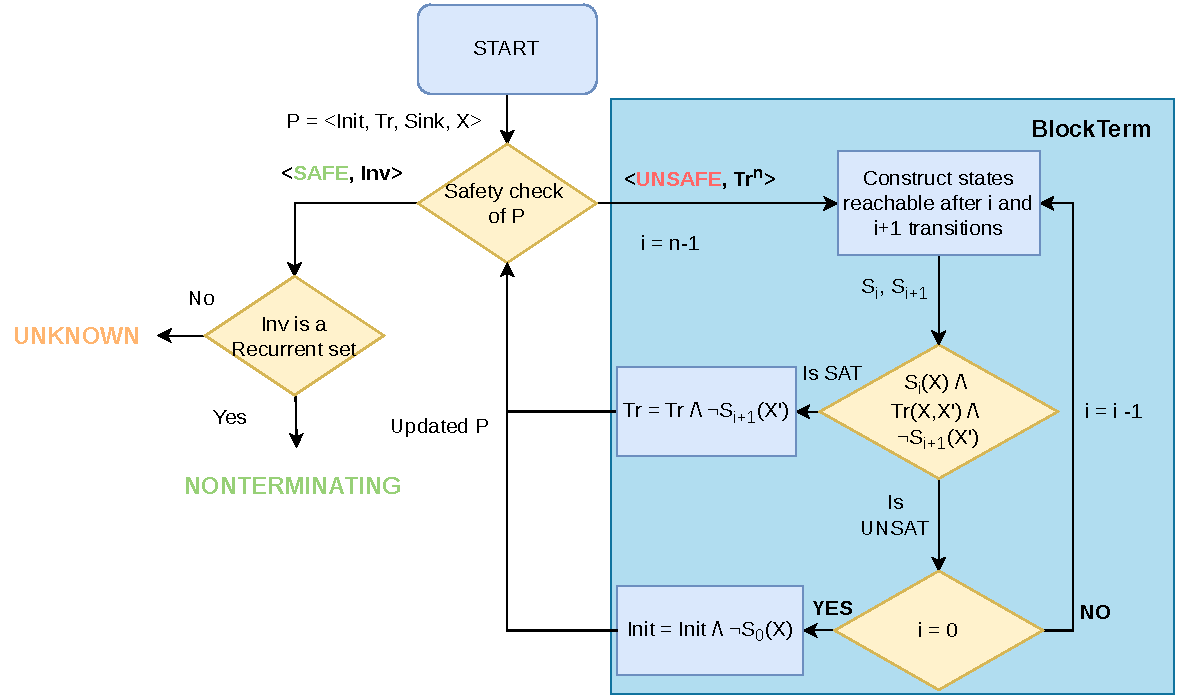
\includegraphics[width=\linewidth]{Figures/SNA.pdf}
    \caption{Execution flow of Safety-based Nontermination analysis, cf~\cite{DBLP:conf/tacas/ChenCFNO14}}
    \label{fig:SNA}
\end{figure}

Algorithm~\ref{Alg:SNA} for Safety-based Nontermination analysis (SNA) takes a 
safety problem $P = \tuple{Init, Tr, \Sink, X}$, where sink states are constructed from TS using
quantifier elimination, $\Sink(X) = \lnot QE(\exists X'. Tr(X,X'))$.
As an output, it returns \NONTERM{} if the system is nonterminating, and \UNKNOWN, if the algorithm cannot conclude the analysis. 
Figure~\ref{fig:SNA} contains the execution flow of Safety-based Nontermination.

\begin{algorithm}[t!]
	\SetInd{0.5em}{0.5em}
    \DontPrintSemicolon
    \small
    \newcommand{\Continue}{\textbf{continue}}
    \caption{Safety-based Nontermination Analysis (SNA), cf~\cite{DBLP:conf/tacas/ChenCFNO14}}
    \label{Alg:SNA}
    \SetKwInOut{Input}{Input}
    \SetKwInOut{Output}{Output}
    \Input{Safety problem $P = \tuple{\Init, \Tr, \Sink, X}$}
    \Output{\NONTERM $\mid$ \UNKNOWN}
    % \SetKwFunction{FAnalyze}{Analyze}
    % \SetKwProg{Fn}{Function}{:}{}
    % \nonl\Fn{\FAnalyze{$P$}}{
        \While{$\top$}{
            $\tuple{\res,\phi = Tr^{n}\ or \Inv} \gets \textsc{SafetyCheck}(P)$\\
            \label{SNA:UNSAFE}\eIf{$\res = \UNSAFE$} {
                $P \gets \blockTerm(P, \phi)$ \label{SNA:BLOCKTERM}
            }
            {
                \If{$\forall X. \phi(X) \rightarrow \exists X'. Tr(X,X')$\label{SNA:SAFE}}{
                    \Return \NONTERM \label{SNA:RECURRENT}
                }
                \Return \UNKNOWN
            }
            
        }
    % }
    
\end{algorithm}
% A

The approach executes a safety check of $P$ in a loop.
At line~\ref{SNA:UNSAFE}, the algorithm handles the case when $P$ is unsafe (i.e., exists a trace reaching sink states).
In this case, the algorithm calls the $\blockTerm$ procedure (Algorithm~\ref{Alg:SNABlock}), which refines the safety problem $P$ by blocking the states that deterministically
lead to the sink states, updating the Safety problem.
$\blockTerm$ is described in detail below.
In the case when $P$ is safe, the algorithm checks if the inductive invariant $Inv(X)$ is a recurrent set (line~\ref{SNA:SAFE}).
The check at line~\ref{SNA:SAFE} is executed using quantifier elimination, checking if the following formula
is unsatisfiable:
$$\exists X. \phi(X) \land \lnot QE(\exists X'. Tr(X,X')).$$
If $Inv(X)$ is a recurrent set, then the transition system is nonterminating.
Otherwise, the algorithm returns \UNKNOWN.

\begin{algorithm}
    \SetInd{0.5em}{0.5em}
    \DontPrintSemicolon
    \small
    \newcommand{\Continue}{\textbf{continue}}
    \caption{\blockTerm(P, $Tr^{n}$), cf~\cite{DBLP:conf/tacas/ChenCFNO14}}
    \label{Alg:SNABlock}
    \SetKwInOut{Input}{Input}
    \SetKwInOut{Output}{Output}
    \SetKwInOut{Data}{Data}
    \Input{Safety problem $P = \tuple{Init, Tr, \Sink, X}$, terminating trace $Tr^{n}(X^{(0)}, \dots, X^{(n)}) = Tr(X^{(0)}, X^{(1)}) \land \dots \land Tr(X^{(n-1)}, X^{(n)})$}
    \Output{Refined safety problem $P'$}
    \Data{$S_0,\dots,S_n$ - formulas which encode states within trace reachable in 0, ..., n transitions}

    % \SetKwFunction{FBlock}{BlockTerm}
    % \SetKwProg{Fn}{Function}{:}{}
    % \Fn{\FBlock{$P, trace$}}{
    \SetAlgoFuncName{BlockTerm}{autoref name}
        $i \gets n-1$ \\
        \While{$i > 0$}{
            $S_{i+1}(X) \gets QE(\exists X^{(0)},\dots, X^{(i)},  X^{(i+2)}, \dots, X^{(n)}.$ $Init(X^{(0)}) \land Tr^{n} \land \Sink(X^{(n)}))[X^{(i+1)} \mapsto X]$ \label{SNA:Si1}\\
            $S_{i}(X) \gets QE(\exists X^{(0)},\dots, X^{(i-1)},  X^{(i+1)}, \dots, X^{(n)}.$ $Init(X^{(0)}) \land Tr^{n} \land \Sink(X^{(n)}))[X^{(i)} \mapsto X]$ \label{SNA:Si}\\
            \If{SAT ? $S_i(X) \land Tr(X,X') \land \lnot S_{i+1}(X')$ \label{SNA:BLOCK}}{
                $Tr'(X,X') \gets Tr(X,X') \land \lnot S_{i+1}(X')$ \label{SNA:TRBLOCK}  \\
                \Return $\tuple{Init, Tr', \Sink, X}$
            }
            $i \gets i - 1$   
        }
        $Init'(X^{(0)}) \gets Init(X^{(0)}) \land \lnot QE(\exists X^{(1)}, \dots, X^{(n)}. Init(X^{(0)}) \land Tr^{n} \land \Sink(X^{(n)}))$  \label{SNA:BLOCKINIT} \\
        \Return $\tuple{Init', Tr, \Sink, X}$
    % }
\end{algorithm}

The $\blockTerm$ procedure takes as input a safety problem $P$ and a trace formula $Tr^{n}(X^{(0)}, \dots, X^{(n)})$ such 
that $Init(X^{(0)}) \land Tr^{n}(X^{(0)}, \dots, X^{(n)}) \land \Sink(X^{(n)})$ is satisfiable.
The algorithm iteratively analyses the transition trace starting from the last transition. 
% It checks if it is possible to take a transition that does not lead to the sink states, starting from the end of the trace.
Algorithm~\ref{Alg:SNABlock} constructs states that are reachable after $i$ and $i+1$ transitions from the initial states using quantifier 
elimination at lines~\ref{SNA:Si1},~\ref{SNA:Si}.
Then, at line~\ref{SNA:BLOCK} it checks if $S_i(X) \land Tr(X,X') \land \lnot S_{i+1}(X')$ is satisfiable, sending a query to the SMT solver.
This query checks if it is possible to reach some state that does not necessarily lead to the sink states.
If it is possible, then the algorithm blocks the states that deterministically lead to the sink states at line~\ref{SNA:TRBLOCK}.
Otherwise, if the trace is deterministic, \blockTerm blocks the subset of initial states that leads to sink (line~\ref{SNA:BLOCKINIT}).


\begin{lemma}\label{Lem:NONTERM}
    If Algorithm~\ref{Alg:SNA} returns NONTERM, then the transition system is nonterminating, cf~\cite{DBLP:conf/vmcai/PodelskiR04}.
\end{lemma}
\begin{example}\label{Ex:SNA}
    Consider a transition system $TS = \tuple{Init, Tr, X}$ with 
    $X = \{x\}$, $Init(X)   \triangleq \top$, and
    $Tr(X, X') \triangleq (x' = x - 1 \lor x' = x - 2) \land x \neq 0$.
    The sink states are $\Sink(x) \triangleq v = 0$, and the initial 
    safety problem is $P = \tuple{Init, Tr, \Sink, x}$.
    This TS is nonterminating, since $x$ can infinitely decrease.

    The execution of Algorithm~\ref{Alg:SNA} updates initial states
    and transition in two iterations of the algorithm, via \blockTerm\: 
    $Init(X) \;\gets\; x \neq 0$, and  $Tr(X, X') \;\gets\; Tr(X, X') \land x' \neq 0$.
    The safety check of the updated problem concludes SAFE,
    with $Inv(X) \triangleq x \neq 0$. 
    $Inv(X)$ is a recurrent set, and algorihtm returns \textsc{NONTERM}.

    \textit{Motivation for transition invariant-based termination analysis.} Consider a 
    small modification (replacing $x\neq0$ with $x>0$): $Tr(X, X') \triangleq 
    (x' = x - 1 \lor x' = x - 2) \land x > 0$. 
    This renders $TS$ terminating, since $x$ is strictly positive and decreases every step. 
    However, Algorithm~\ref{Alg:SNA} cannot detect termination by design, and 
    it would return \UNKNOWN. 

    Let us examine the execution of Algorithm~\ref{Alg:SNA} on this example.
    First, using \blockTerm, it blocks initial states that instantly terminate:
    $Init(X) \;\gets\; x > 0$.
    In the second iteration, \textsc{SafetyCheck}$(P)$ returns UNSAFE with a 
    trace $Tr^1(X^{(0)}, X^{(1)})$, detecting that $\exists X^{(0)}, X^{(1)}. 
    Init(X^{(0)}) \land Tr^1(X^{(0)}, X^{(1)}) \land \lnot \Sink(X^{(1)})$.
    Our key insight is to generalise such traces into a formula, describing an 
    entire class of terminating behaviours. 
    If this generalisation yields a disjunctively well-founded 
    transition invariant over all reachable states, it witnesses 
    termination.
    Particularly, $\TrInv(X, X') \triangleq x' < x \land x > 0$ is a well-founded transition 
    invariant which proves the termination of $TS$.
    Section~\ref{sec:Main} presents the algorithm that automates this generalisation via 
    Craig interpolation.
\end{example}

%

\section{Termination Analysis via Interpolation-based Transition Invariant Generation}

We propose a new approach for proving termination that leverages safety verification to generate a well-founded transition invariant
candidate via interpolation.
At each iteration, our procedure constructs a trace from the initial states to a sink state.
A well-founded transition invariant is then constructed based on the overapproximation of the terminating trace.
If the invariant is valid for all reachable states, termination is concluded. 
The interpolation-based approach enables efficient property-directed transition invariant generation, as it is constructed with respect to the termination condition.

\subsection{Interpolation-based Generation of Well-Founded Transition Invariants}

The core of our approach is the procedure for automated, interpolation-based generation of 
well-founded transition invariants: \trInvSynthesis. 
Given a transition system and a terminating trace, the procedure 
constructs a disjunctively well-founded approximation of the transition trace. 
If the resulting formula constitutes a transition invariant over all reachable states, 
it witnesses termination.

The Procedure consists of five major steps:
% (1) computing $T^n$, the formula encoding states that terminate within $n$ transitions.
% $T^n$ is used to construct the interpolant. It guarantees that no states other then $Sink$ are reachable in $n$ transitions; 
(1) computing $NT^n$, the formula encoding states that do not necessarily terminate within $n$ transitions.
$NT^n$ is used to construct the interpolant. The negation of $NT^n$ defines the states that necessarily reach $Sink$ 
in at most $n$ transitions; 
(2) constructing an over-approximation of the terminating trace via interpolation. 
The usage of sink states allows the interpolant to capture the reason for termination; 
(3) converting the interpolant into an underapproximating DNF formula.
This allows to efficiently synthesise ranking functions for separate disjuncts; 
(4) filtering disjuncts to retain only those encoding well-founded relations, constructing a candidate transition invariant.
Only well-founded relations are saved, as transition invariant needs to be disjunctively well-founded to witness termination; and 
(5) computing the formula encoding states for which candidate formula is a valid transition invariant.
Transition invariant needs to be valid only over the reachable states to conclude termination.
Therefore, if all reachable states satisfy this formula - TS is terminating.
The overall flow of the procedure is illustrated in the Figure~\ref{fig:TrInvGen}.

\begin{figure}[t]
    \centering
    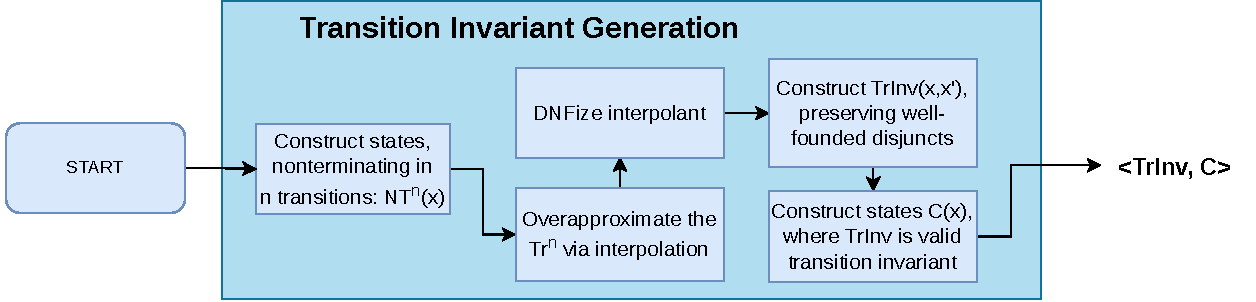
\includegraphics[width=\linewidth]{Figures/TrInv.pdf}
    \caption{Execution Flow of Interpolation-based Transition Invariant Generation}
    \label{fig:TrInvGen}
\end{figure}


\begin{algorithm}[t!]
	\SetInd{0.5em}{0.5em}
    \DontPrintSemicolon
    \small
    \newcommand{\Continue}{\textbf{continue}}
    \caption{$\trInvSynthesis(P, Tr^n, TInv)$.}
    \label{Alg:SNA_TrInv}
    \SetKwInOut{Input}{Input}
    \SetKwInOut{Output}{Output}
    \Input{Safety problem $P = \tuple{Init, Tr, Sink, X}$, transition trace $Tr^n(X^{(0)}, X^{(1)}, \dots, X^{(n)})$, candidate transition invariant $TInv(X,X')$}
    \Output{Updated transition invariant $TInv(X,X')$ and formula $C(X)$ encoding states covered by
    transition invariant}
    $NT^n(X^{(0)}) \gets  QE(\exists X^{(1)}, \dots, X^{(n)}.$ $Tr^{n}(X^{(0)}, X^{(1)}, \dots, X^{(n)}) \land \lnot Sink(X^{(n)}))$ \label{SNA_TrInv:T} \\
    % $T^n(X^{(0)}) \gets \lnot QE(\exists X^{(1)}, \dots, X^{(n)}.$ $Tr^{n}(X^{(0)}, X^{(1)}, \dots, X^{(n)}) \land \lnot Sink(X^{(n)}))$ \label{SNA_TrInv:T} \\
    % $itp(X,X') \gets Itp(Tr^{n}(X, \dots, X'), T^n(X) \land \lnot Sink(X'))$\label{SNA_TrInv:Itp}\\
    $itp(X,X') \gets Itp(Tr^{n}(X, \dots, X'), \lnot NT^n(X) \land \lnot Sink(X'))$\label{SNA_TrInv:Itp}\\
    $Cs(X,X') \gets toDNF(itp)$ \label{SNA_TrInv:toDNF}\\
    $TInv \gets TInv \lor \bigvee_i \{d_i \in Cs| \text{$\exists$ ranking function $f(X)$} \}$\label{SNA_TrInv:TINV} \\
    $C(X) \gets \lnot QE(\exists X',X''.$ $\bigl(Id(X,X') \lor TInv(X,X')\bigr)  \land Tr(X',X'') 
        \land \lnot TInv(X,X''))$ \label{SNA_TrInv:NC} \\
    \Return $\tuple{TInv, C}$
\end{algorithm}

Algorithm~\ref{Alg:SNA_TrInv} takes as an input a safety problem $P = \tuple{Init, Tr, Sink, X}$,
a transition trace $Tr^n(X^{(0)}, X^{(1)}, \dots, X^{(n)})$, and a transition invariant formula $TInv(X,X')$. 
It returns a tuple of formulas $\tuple{TInv, C}$, where $TInv(X,X')$ is a disjunctively well-founded transition invariant 
candidate, and $C(X)$ is a formula encoding the states for which $TInv$ is a valid transition invariant. 
It proceeds in the following steps:
% Define from the negation, not the itself

\textbf{Step 1}: \textit{Computing $NT^n$ (line~\ref{SNA_TrInv:T}).} 
$NT^n(X)$ encodes all states that do not necessarily terminate in $n$ 
transitions, is defined by the following property:
% $NT^n(X)$ encodes all states guaranteed to reach a sink state within $n$ 
% transitions, is defined by the following property:

$$\exists X^{(0)}, \dots, X^{(n)}. Tr^{n}(X^{(0)}, \dots, X^{(n)}) \land \lnot Sink(X^{(n)})$$

$NT^n$ is constructed with quantifier elimination, eliminating all variables from the formula except for $X^{(0)}$.
Construction of $NT^{(n)}$ enables the overapproximation of the trace. 

\begin{example}\label{Ex:Tn}
    % Consider $TS = \tuple{Init, Tr, X}$ with $Init \triangleq  x > 0$, $Tr(X,X') \triangleq  ((x' = x - 1 \lor x' = x - 2) \land x > 0) \lor (x < -10 \land x' = x - 1)$, $X \triangleq  \{x\}$.
    % For $n = 2$ quantifier elimination would yield $T^2(X) = x \leq 2$.
    % States with $x \in \{3,4\}$ can reach $Sink$ in two transitions but are 
    % not guaranteed to do so, so they are not included in $T^2$.
    % States with $x \in \{1,2\}$ terminate in 1 or 2 transitions.
    Consider $TS = \tuple{Init, Tr, X}$ with $Init \triangleq  x > 0$, $Tr(X,X') \triangleq  ((x' = x - 1 \lor x' = x - 2) \land x > 0) \lor (x < -10 \land x' = x - 1)$, $X \triangleq  \{x\}$.
    In this TS, sink states can be encoded as $Sink(X) \triangleq x \leq 0 \land x \geq -10$.
    For $n = 2$ quantifier elimination would yield $NT^2(X) = x > 2$.
    States with $x \in \{3,4\}$ can reach $Sink$ in two transitions, but not necessarily.
    Therefore these states are included in $NT^2$.
\end{example}

\textbf{Step 2}: \textit{Interpolation (line ~\ref{SNA_TrInv:Itp}).}
The following formula is unsatisfiable by construction, since any state in 
$\lnot NT^n$ must reach $Sink$ within $n$ steps:

$$\lnot NT^{n}(X^{(0)}) \land Tr^{n}(X^{(0)}, \dots, X^{(n)}) \land \lnot Sink(X^{(n)})$$

This allows to compute the \textbf{Craig interpolant}, which over-approximates the trace $Tr^{n}$.
Crucially, the usage of the sink states for interpolant construction allows the interpolant to capture the reason \emph{why} 
the particular trace is terminating.



\textbf{Step 3}: \textit{DNF underapproximation (line ~\ref{SNA_TrInv:toDNF}).}
For a transition invariant to witness termination, it must be 
disjunctively well-founded, meaning every disjunct must encode a 
well-founded relation. Converting the interpolant to a full DNF 
would make each disjunct a conjunction, simplifying the 
well-foundedness check, but full DNF conversion can cause an 
exponential blowup in formula size. Moreover, even a complete DNF 
is not guaranteed to yield a transition invariant or to witness 
termination.

Instead, our algorithm follows a lazy approach: it constructs an 
under-approximating DNF formula on demand. 
Concretely, algorithm constructs disjuncts as follows:
(1) SMT solver prodices a model that satisfies $itp$, (2) 
Using produced model, the satisfied literals are extracted from the SMT formula and conjoined,
(3) This conjunction is one of the dinsjuncts in the constructed DNF. It is blocked from the itp, 
and the dnfization proceeds (until reaching certain limit).
The result is a formula:
$$Cs(X,X') \triangleq \bigvee_{i=0}^m d_i$$
where each $d_i$ is a conjunction, and $Cs(X,X') \rightarrow itp(x,x')$.
This approach significantly reduces formula size and speeds up both DNFization and 
subsequent well-foundedness check, while preserving correctness: 
in the worst case, $Cs$ fails to be a transition invariant over all 
reachable states, but this is equally possible even with a complete DNF conversion.
% Empirically, bounding the number of disjuncts produces more 
% compact and efficiently verifiable termination proofs.
% Our algorithm produces a model satisfying the SMT formula.
% Using produced model, it extracts the satisfied literals from the SMT formula, and constructs a conjunction of these literals.
% This conjunction is one of the dinsjuncts in the constructed DNF. This conjunction is blocked in the original formula, and the process proceeds.
% It allows to significantly reduce the size of the resulting formula and speed up the DNF conversion, while preserving correctness: 
% in the worst case, the resulting formula is not a transition invariant (which can happen even if the complete DNF is produced).
% Empirically, we observed that limiting the number of disjuncts results in more size-efficient and quick termination proofs.
% The execution of the procedure returns a formula:

% The number of disjuncts is bounded by a constant (a tunable parameter depending on the available size of RAM), since DNF 
% conversion can cause an exponential blowup in formula size.  Move to implementation & evaluation
% Bring citation 3 to background section

\textbf{Step 4}: \textit{Filtering Well-Founded Disjuncts (line ~\ref{SNA_TrInv:TINV}).}
For each disjunct $d(X,X') \in Cands(X,X')$ algorithm checks if $d(X,X')$ encodes a well-founded relation.
Our technique uses automated linear ranking function synthesis~\cite{DBLP:conf/vmcai/PodelskiR04} for checking the existence of a ranking function.
The disjuncts for which a ranking function exists are preserved, and the rest are discarded.
The resulting formula is disjoined with the input candidate transition invariant $TInv$.

\textbf{Step 5}: \textit{Synthesis of the states for which transition invariant is valid (line ~\ref{SNA_TrInv:NC}).}
If $TrInv$ is a transition invariant over all reachable states, then TS terminates, since every disjunct corresponds to well-founded relation.
To verify this, procedure computes the formula $C(X)$ encoding the states over which $TrInv$ is a valid transition invariant. 
% Split this thing into 2 properties
% Make it consistent with the code
\begin{definition}[Coverage formula]
    Consider a transition system $TS = \tuple{Init, Tr, X}$ and a formula $TrInv(X,X')$. 
    We say that $C(X)$ is a coverage formula, if the following properties hold $\forall X, X',X''$:
    \begin{align*}
     C(X) \land Tr(X,X') \rightarrow& TrInv(X,X') \\
     C(X) \land TrInv(X,X') \land Tr(X',X'') \rightarrow& TrInv(X,X'')
    \end{align*}
    Meaning, that $TrInv$ is a transition invariant over states satisfying $C(X)$.
\end{definition}

Similarly to $NT^{n}$, $C(X)$ is constructed by applying quantifier elimination, negating the states for 
which $TrInv$ is not a transition invariant.
% example has an issue!
\begin{example}~\label{Ex:C}
    Continuing Example~\ref{Ex:Tn}, suppose the procedure constructs 
    $TrInv \triangleq x' < x \land x' \geq 0$. Quantifier elimination then
    yields $C(X) \equiv x > 0$.
\end{example}

\emph{Note.} If $\lnot C(X)$ is not reachable, then $TrInv(X,X')$ is a disjunctively well-founded
transition invariant over all reachable states, and witnesses the termination of transition system.
For illustration, transition invariant in the Example~\ref{Ex:C} is sufficient to prove termination, 
since $\lnot C(X) \triangleq x \leq 0$ is the sink states, and for all other states $TrInv$ is a valid
transition invariant.

\begin{lemma}\label{Lem:Term}
    Let $TS = \tuple{Init, Tr, X}$ be a transition system and let 
    $C(X)$ be a formula such that $\lnot C(X)$ is unreachable in 
    $TS$. If $TrInv(X,X')$ is a finite disjunction of formulas encoding well-founded
    relations and satisfies $\forall X, X',X''$:
    \begin{align*}
     C(X) \land Tr(X,X') \rightarrow& TrInv(X,X') \\
     C(X) \land TrInv(X,X') \land Tr(X',X'') \rightarrow& TrInv(X,X'')
    \end{align*}    
    then $TS$ is terminating.
\end{lemma}
\begin{proof}
    We show that $TrInv$ is a disjunctively well-founded transition 
    invariant over the reachable states of $TS$, from which 
    termination follows by~\cite{DBLP:conf/lics/PodelskiR04}.

    \textbf{Disjunctive well-foundedness.} By construction, for each disjunct 
    $d_i$ of $TrInv = \bigvee_i d_i$ there exists a ranking function.
    Therefore, every disjunct is a logical encoding of 
    well-founded relation~\cite{DBLP:conf/vmcai/PodelskiR04}. 
    Hence $TrInv$ is disjunctively well-founded.

    \textbf{Transition invariant.} We show that 
    $\forall X,X'.\ R(X) \land Tr^+(X,X') \rightarrow TrInv(X,X')$,
    where $R(X)$ denotes the reachable states of $T$, by induction 
    on the number of steps $n$ in $Tr^+(X,X')$.

   \emph{Base case} ($n = 1$): It is needed to prove that:
   $$R(X) \land Tr(X,X') \rightarrow TrInv(X,X')$$ 
    Since $\lnot C(X)$ is unreachable, $R(X) \rightarrow C(X)$. 

    The following assumption holds by the lemma statement:
    $$C(X) \land Tr(X,X') \rightarrow TrInv(X,X').$$
    Since $R(X) \rightarrow C(X)$, therefore $R(X) \land Tr(X,X') \rightarrow C(X) \land Tr(X,X')$,
    the base case holds.

   \emph{Inductive step}: Assume $R(X) \land Tr^n(X, \dots,X') \rightarrow 
    TrInv(X,X')$ for some $n \geq 1$. 
    Let $Tr^{n+1}(X,X'')$ hold, so there $\exists X, \dots, X', X''. R(X) \land Tr^n(X, \dots, X') \land Tr(X',X'')$. 
    Since $R(X) \land Tr^n(X, \dots, X') \rightarrow TrInv(X,X')$, then trivially
    $R(X) \land Tr^n(X,X') \land Tr(X',X'') \rightarrow R(X) \land TrInv(X,X') \land Tr(X',X'')$.
    Now, due to the fact that $R(X) \rightarrow C(X)$, the following holds:
    $R(X) \land TrInv(X,X') \land Tr(X',X'') \rightarrow C(X) \land TrInv(X,X') \land Tr(X',X'').$
    And by claim in the lemma:
    $$C(X) \land TrInv(X,X') \land Tr(X',X'') \rightarrow TrInv(X,X'').$$

    Therefore, through the chain of implications, we have:
    $$R(X) \land Tr^{n+1}(X,X') \rightarrow TrInv(X,X').$$

    Thus $TrInv$ is a disjunctively well-founded transition 
    invariant over all reachable states, and $TS$ is 
    terminating.
\end{proof}

%-----------------------------------------------------------------------
\subsection{Interpolation-based Termination Analysis}
%-----------------------------------------------------------------------


This subsection presents the full termination analysis procedure, using the interpolation-based transition invariant generation.
It integrates \trInvSynthesis into the safety-based analysis loop of Algorithm~\ref{Alg:SNA}.
At each iteration, instead of only blocking terminating states, the algorithm also constructs a transition invariant 
candidate. 
The overall flow is shown in Figure~\ref{fig:SNATrInv}.
 
\begin{figure}[t]
    \centering
    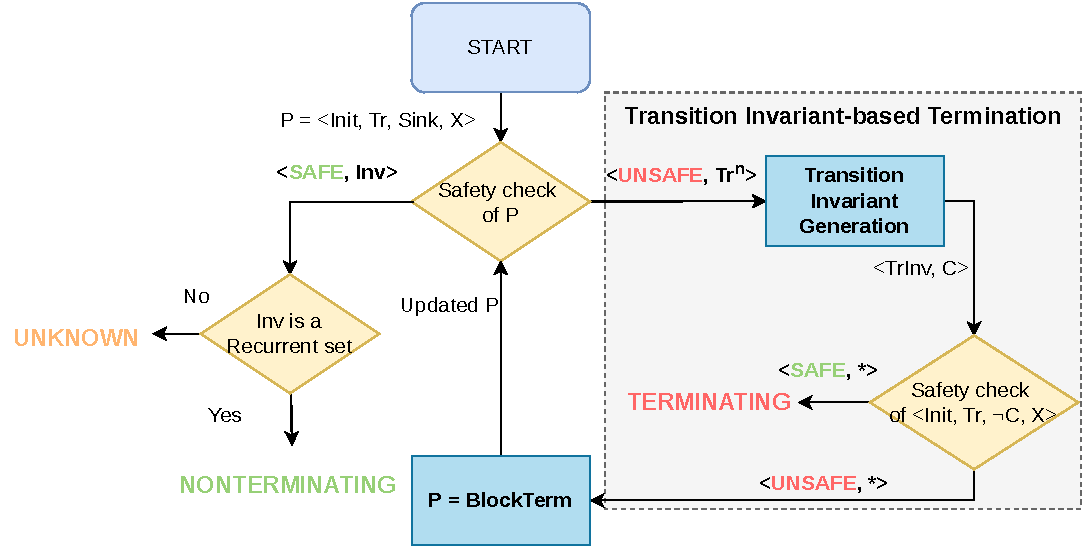
\includegraphics[width=\linewidth]{Figures/SNA+T.pdf}
    \caption{Execution Flow of Interpolation-based Transition Invariant Generation (New components are placed in a grey block, lines~\ref{SNA_Term:Synth},\ref{SNA_Term:CheckNc},\ref{SNA_Term:NEWTERM}).}
    \label{fig:SNATrInv}
\end{figure}

%  Notation is confusing, replace everything with phis, no need for phi'
%  On the second safety check use *
\begin{algorithm}[t!]
	\SetInd{0.5em}{0.5em}
    \DontPrintSemicolon
    \small
    \newcommand{\Continue}{\textbf{continue}}
    \caption{Interpolation-based Transition Invariant Generation for Proving and Disproving Termination.}
    \label{Alg:SNA_Term}
    \SetKwInOut{Input}{Input}
    \SetKwInOut{Output}{Output}
    \SetKwInOut{Data}{Data}
    \Input{Safety problem $P = \tuple{Init, Tr, Sink, X}$}
    \Output{TERM $\mid$ NONTERM $\mid$ UNKNOWN}
    \Data{$TInv$ - formula that encodes transition invariant}
    $TInv \gets \bot$ \\
    \While{$\top$} {
        \label{SNA_Term:Safety} $\tuple{res, \phi = Tr^n\ or\ Inv} \gets safetyCheck(P)$ \\
        \eIf{$res = UNSAFE$} {
            $\tuple{TInv, C} \gets \trInvSynthesis(P, Tr^n, TInv)$ \label{SNA_Term:Synth} \\
            $\tuple{res', \_} \gets safetyCheck(\tuple{Init, Tr, \lnot (C \lor Sink), X})$ \label{SNA_Term:CheckNc} \\
            \eIf{$res' = UNSAFE$} {
                $P \gets \blockTerm(P, \phi)$\label{SNA_Term:BlockTerm} \\
            }
            {
               \Return $TERM$\label{SNA_Term:NEWTERM}
            }
        }{
            \lIf{$\forall X. \phi(X) \rightarrow \exists X'. Tr(X,X') \land \phi(X')$} {
                \Return $NONTERM$ \label{SNA_Term:NONTERM}
            }
            \Return UNKNOWN
        }
        
    }
\end{algorithm}


The Algorithm~\ref{Alg:SNA_Term} takes as input a Safety Problem $P=\tuple{Init, Tr, Sink, X}$, where $Init$ and 
$Tr$ encode the initial states and transition relation, $Sink$ is the formula encoding sink states, and $X$ is 
a set of variables over which the Transition System is defined.
As an output, the algorithm returns NONTERM if TS is nonterminating, TERM if it is terminating, and UNKNOWN if the procedure 
cannot determine the final result.
The procedure maintains a formula encoding a candidate transition invariant $TInv(X,X')$ .
During the execution, $TInv$ is extended with new disjuncts, which are generated by the \trInvSynthesis procedure, and encode well-founded relations. 
Changes to the original SNA are in the lines~\ref{SNA_Term:Synth},~\ref{SNA_Term:CheckNc}, and ~\ref{SNA_Term:NEWTERM}.


Algorithm commences by analyzing the original safety problem.
Every iteration, similarly to the Algorithm~\ref{Alg:SNA}, begins with the safety check at line~\ref{SNA_Term:Safety}.
The algorithm handles two possible cases:

\paragraph{UNSAFE.} A terminating trace $Tr^n$ exists.
The algorithm calls 
\trInvSynthesis\ to extend $TInv$ and compute the coverage formula $C(X)$ (line~\ref{SNA_Term:Synth}).
\konst{Think how to include sink states to C(x), bc it does not make sense for TrInv to be valid over Sink(x).}
Then, it checks if $\lnot (C(X) \lor Sink(X))$ is reachable from the initial states (line~\ref{SNA_Term:CheckNc}).
If $\lnot (C(X) \lor Sink(X))$ is reachable, algorithm refines the safety problem by blocking 
the states deterministically leading to termination via \blockTerm, and the loop continues.
Otherwise, $TInv$ is a transition invariant over all reachable states, and algorithm concludes termination.

\paragraph{SAFE.} No sink state is reachable. 
If $\phi(X)$ is a recurrent set, the system is nonterminating. 
Otherwise, the algorithm returns UNKNOWN as the analysis is inconclusive.

\begin{example}
    Consider $TS$ from Example~\ref{Ex:Tn} with 
    $Init \triangleq x > 0$, 
    $Tr \triangleq \bigl((x'=x-1 \lor x'=x-2) \land x>0\bigr) 
    \lor \bigl(x<-10 \land x'=x-1\bigr)$, $X \triangleq \{x\}$.

    Preprocessing computes 
    $Sink \equiv x \leq 0 \land x \geq -10$.
    Then, the algorithm is called with $P=\tuple{Init, Tr, Sink, X}$.

    %

    The safety check detects a trace $Tr^1$ reaching $Sink$. 
    \trInvSynthesis produces a transition invariant candidate $TInv(X,X') \triangleq x' < x \land x' \geq 0$ and the formula $C(X) = x > 0$.
    The safety check for $\tuple{Init, Tr, \lnot (C(X) \lor Sink(X)), x}$ returns SAFE, and algorithm concludes that the transition system is terminating.
\end{example}


%-----------------------------------------------------------------------
\subsection{Correctness}
%-----------------------------------------------------------------------


This subsection proves the soundness of the introduced approach. We first prove that when algorithm returns TERM, the transition system is nonterminating,
and then we prove the correctness of the nontermination.
%  Add well-foundness definition

\begin{lemma}
    If Algorithm~\ref{Alg:SNA_Term} returns $TERM$, then the transition system $\tuple{Init, Tr, X}$ is terminating.
\end{lemma}
\begin{proof}
    $TERM$ is returned only at the line~\ref{SNA_Term:NEWTERM}, of the algorithm.
    It means that there exists a transition invariant $TInv$ which is valid over states $C(X)$, and $\lnot C(X)$ is 
    unreachable from the initial states.
    The safety problem is updated iteratively, blocking the states that deterministically lead to the termination,
    so in the end the $P = \tuple{Init', Tr', Sink, X}$, where $Init'(X) = Init(X) \land \bigwedge_{i=0}^{m} \lnot S_i(X)$
    and $Tr' = Tr(X) \land \bigwedge_{i=0}^{l} \lnot S_j(X')$ .
    According to the Lemma~\ref{Lem:Term}, Transition System $\tuple{Init', Tr', X}$ is terminating, since $TInv$ is a disjunctively well-founded
    transition invariant over all reachable states.

    Since the states satisfying $\bigvee_{i=0}^{m} S_i(X)$ and $\bigvee_{i=0}^{l} S_j(X')$ deterministically lead to the termination,
    every trace of $\tuple{Init, Tr, X}$ either follows $Tr'$ or passes through a blocked state which leads to termination.
    Hence $\tuple{Init, Tr, X}$ is terminating.
\end{proof}


\begin{lemma}
    If Algorithm~\ref{Alg:SNA_Term} returns $NONTERM$, then the transition system $\tuple{Init, Tr, X}$ is nonterminating.
\end{lemma}
\begin{proof}
    The proof of this lemma follows directly from the Lemma~\ref{Lem:NONTERM}, as the nontermination proof procedure 
    directly corresponds to one described in the Algorithm~\ref{Alg:SNA}. 
\end{proof}



\begin{example}\label{Ex:Motivation}
    Consider a transition system $TS = \tuple{Init, Tr, X}$ with 
    $X = \{x, u\}$, where $x, u$ are integer variables, $Init(X)   \triangleq u < 10 \land x > 0 $, and
    $Tr(X, X') \triangleq ((x' = x - 1 \land u' = u ) \lor (x' = x + 1 \land u' = u + 1 \land u < 10)) \land x > 0$.


    Intuitively, at each step the system either decrements $x$ (and keeps $u$ unchanged), or increments both $x$ and $u$ 
    provided $u < 10$. 
    Once $u = 10$, only the decrementing branch is available, and $x$ decreases monotonically to zero. 
    Hence $TS$ is terminating.
    The sink states are $Sink(X) \triangleq x \leq 0$.
    The initial safety problem is $P = \tuple{Init, Tr, Sink, X}$.

    \textit{Iteration 1.} $safetyCheck(P)$ returns UNSAFE with a trace $Tr^1(X^{(0)}, 
    X^{(1)})$: a sink state is reachable in one transition via the 
    decrement when $x = 1$.
    \trInvSynthesis\ constructs transition invariant:
    $TInv(X, X') \;\triangleq\; x' < x \land x > 0$. 
    The coverage formula is then computed as: $C(X) \;\triangleq\; u = 10$.
    The safety check for $\tuple{Init, Tr, \lnot C, X}$ returns UNSAFE, since states 
    with $u < 10$ are reachable from $Init$. 
    The algorithm therefore calls \blockTerm, blocking the sink-reaching 
    transition:
    $$Tr(X, X') \;\gets\; Tr(X, X') \land x' > 0 .$$

    \textit{Iteration 2.} $safetyCheck(P)$ returns SAFE with inductive invariant 
    $Inv(X) \equiv x > 0$. 
    Since $x = 1 \land u = 10$ has no  outgoing transition under the refined $Tr'$ (the decrementing 
    branch would produce $x' = 0$, which is now blocked), $Inv$ is not a recurrent set. 
    Algorithm~\ref{Alg:SNA_Term} returns \textsc{Unknown}.

    \textbf{The limitation.} The root cause why algorithm cannot prove termination is that $TInv$ does 
    not cover states with $u < 10$. 
    It captures why the system terminates when $u = 10$, but not the global argument: $u$ 
    grows until at most $u = 10$, after which $x$ decreases monotonically. 
    A complete termination proof requires a \emph{second} disjunct covering the $u < 10$ region.
    Below, we propose an extension which would allow to concentrate on the state space
    which is not covered by transition invariant.
\end{example}


\section{Extended Interpolation-based Transition Invariant Generation for Proving and Disproving Termination}
\label{Sec:Main}

Algorithm~\ref{Alg:SNA_Term} is already capable of proving termination efficiently through the construction of transition invariants.
This section describes an extension of the algorithm that aims to achieve better interaction between termination and nontermination
analysis.
Additionally, we present further extensions to the original SNA algorithm that improve overall performance. 
The high-level flow of the extended algorithm can be seen in Figure~\ref{fig:SNA++}.

\subsection{Utilising States for Which Transition Invariant is not Valid}~\label{Sec:Refinement}

Constructed transition invariant candidate can be used to guide the termination analysis.
Particularly, the Algorithm~\ref{Alg:SNA_Term} constructs the formula $C(X)$ encoding states for which the transition invariant is valid.
If $\lnot C(X)$ is reachable, it means that there exist states for which the transition invariant is not valid, and which potentially can lead to non-termination.
The intuition is to compute the reachable states $S_m$ within $\lnot C(X)$ (which corresponds to line~\ref{SNA_Refined:Sm} of Algorithm~\ref{Alg:SNA_Refined}).
Then, to attempt either prove termination or nontermination of these particular states within considered transition system (line~\ref{SNA_Refined:PushNewProblem}).


In the case of termination, the algorithm produces a witness transition invariant that extends the transition invariant of the original
system, covering previously uncovered states.
Otherwise, if nontermination is proven for $S_m$, then the original TS is also nonterminating, since $S_m$ is reachable from the initial states.


\begin{figure}[t]
    \centering
    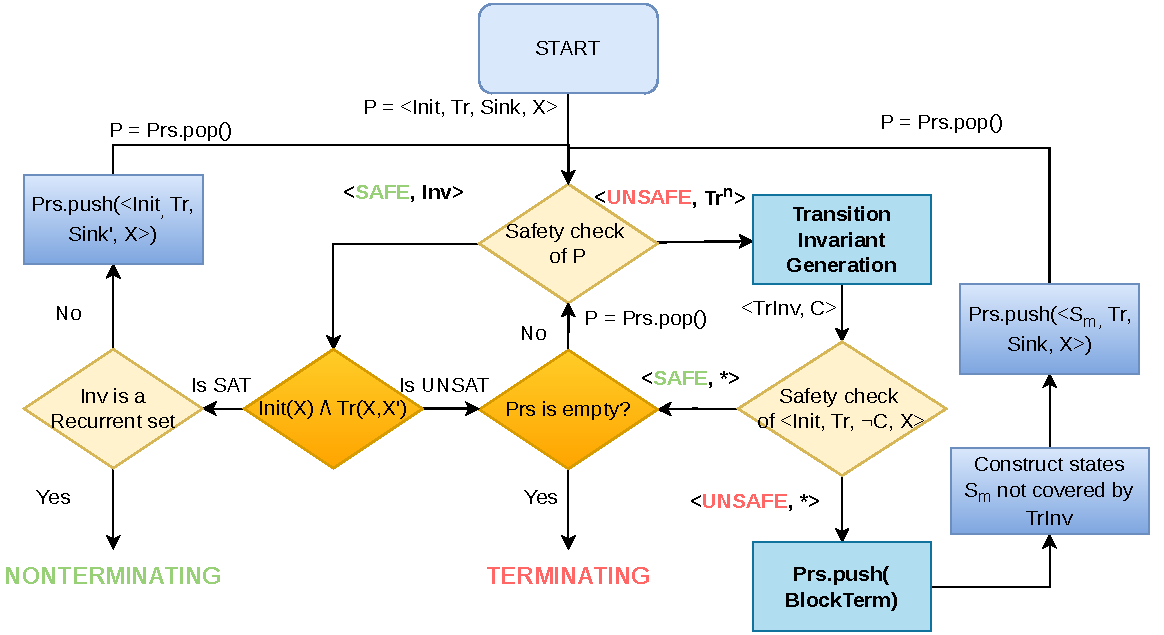
\includegraphics[width=\linewidth]{Figures/SNA++.pdf}
    \caption{Optimized Interpolation-based Termination Analysis (New components are highlighted in dark orange and dark blue colours).}
    \label{fig:SNA++}
\end{figure}

\subsection{Full Algorithm}

% Mention that A and B can be used for Algo 1
% Make people understand that C is much more important!!! Example to motivate each section!!!
% The optimized version of the algorithm is similar to the Algorithm~\ref{Alg:SNA_Term}.
% Main differences are the refinement of the safety problem, and the check for trivial termination.
% These changes allow to significantly improve the overall power and performance of the algorithm.
% In the description, we would concentrate particularly on the changes in the flow, as the rest of the algorithm is quite similar.
% Description in the line 10 - maybe explicit else - continue.

\begin{algorithm}[t!]
	\SetInd{0.5em}{0.5em}
    \DontPrintSemicolon
    \small
    \newcommand{\Continue}{\textbf{continue}}
    \caption{Extended Interpolation-based Transition Invariant Generation for Proving and Disproving Termination.}
    \label{Alg:SNA_Refined}
    \SetKwInOut{Input}{Input}
    \SetKwInOut{Output}{Output}
    \SetKwInOut{Data}{Data}
    \Input{Safety problem $P = \tuple{Init, Tr, Sink, X}$}
    \Output{TERM $\mid$ NONTERM}
    \Data{$TInv$ - formula that encodes transition invariant, $Prs$ - stack of Safety Problems to be
    analyzed for termination}
    $TInv \gets \bot$ \\
    $Prs \gets [P]$ \label{SNA_Refined:Prs} \\
    \While{$\top$} {
        \label{SNA_Refined:Extension} $\tuple{Init', Tr', Sink', X} \gets Prs.pop()$ \\
        \label{SNA_Refined:Safety} $\tuple{res, \phi = Inv\ or\ Tr^n} \gets safetyCheck(\tuple{Init', Tr', Sink', X})$ \\
        \eIf{$\tuple{res, \phi} = \tuple{UNSAFE, Tr^{n}(X^{(0)}, \dots, X^{(n)})}$} {
            $\tuple{TInv, C} \gets \trInvSynthesis(P, \phi, TInv)$ \\
            \label{SNA_Refined:CheckNc} $\tuple{res', \_} \gets safetyCheck(\tuple{Init', Tr', \lnot C, X})$ \\
            \eIf{$res' = SAFE$} {
                \eIf {$Prs = \emptyset$} {\Return $TERM$\label{SNA_Refined:NEWTERM}}
                {\Continue}
            }
            {
                $Prs.push(\blockTerm(P', \phi))$ \\
                $S_m \gets QE(\exists X^{(0)}, \dots, X^{(m-1)}, Init(X^{(0)}) \land Tr^m(X^{(0)}, \dots, X^{(m)}) \land \lnot C(X^{(m)}))$ \label{SNA_Refined:Sm}\\
                $Prs.push(\tuple{S_m, Tr', Sink', X})$\label{SNA_Refined:PushNewProblem}
            }
        }{
        %    \label{SNA_TERM:SAFE}
            \lIf{$\forall X. \phi(X) \rightarrow \exists X'. Tr'(X,X') \land \phi(X')$} {
                \Return $NONTERM$ \label{SNA_Refined:RECURRENT}
            } 
            \eIf {UNSAT ? $\phi(X) \land Tr'(X,X')$} {
                    \lIf{$Prs = \emptyset$} {\Return $TERM$ \label{SNA_Refined:TERM}}
            } {
                $Sink'(X) \gets \lnot QE(\exists X'. Tr'(X,X'))$ \label{SNA_Refined:Refinement} \\ 
                $Prs.push(\tuple{Init', Tr', Sink', X})$
            }
        }
        
    }
\end{algorithm}


Algorithm~\ref{Alg:SNA_Refined} extends Algorithm~\ref{Alg:SNA_Term} to enable more efficient termination and nontermination proving. 
\konst{Think about algo $Tr^m$ appears from nowhere.}
First, in addition to maintaining the transition invariant,
the algorithm maintains a stack of safety problems to be analyzed: $Prs$ (line~\ref{SNA_Refined:Prs}).
At each iteration, the algorithm pops a safety problem from the stack and analyzes it.
The stack allows the algorithm to focus on the termination analysis of particular reachable states within 
the TS.
The original safety problem always remains in the $Prs$ stack with blocked states that deterministically lead to termination.

The postprocessing phase of transition invariant construction is the main change to the Algorithm~\ref{Alg:SNA_Term}.
When $\lnot C$ is reachable, the extended algorithm performs two key actions: (1) it pushes the $\blockTerm$-refined problem 
(as in the original algorithm), and (2) it additionally pushes a new subproblem where  
states not covered by the transition invariant ($S_m$, line~\ref{SNA_Refined:PushNewProblem}) serve as the initial states. 
This approach allows the algorithm to concentrate on proving termination or nontermination for particular reachable states, rather than necessarily proving termination for the entire system.

Otherwise, if $\lnot C$ is not reachable, $TInv$ proves termination of the currently analyzed TS (which may be a refined TS 
previously pushed onto the stack), and the number of remaining subproblems decreases.

The following subsections describe two additional optimizations that further enhance algorithm performance:



\textit{Simple termination check.} When the safety check returns SAFE and $Inv(X)$ is not a recurrent set, 
the algorithm can additionally check whether it is possible to take a transition from the initial states by querying:
$$Init(X) \land Tr(X,X')$$
If this formula is unsatisfiable, then no transition can be taken from the initial states (or all transitions are blocked, 
meaning all reachable states deterministically lead to termination), and the system is trivially terminating. 
This check is implemented at line~\ref{SNA_Refined:TERM}.


\textit{Refinement of Recurrent sets.} When $Inv(X)$ is not a recurrent set, this is often because \blockTerm\ 
has eliminated all transitions leading to $Sink$.
This means that produced $Inv$ contains sink states itself, due to the updated $Tr$. 
New sink states can be computed as:

$$Sink'(X) = \lnot QE(\exists X'. Tr'(X,X'))$$

The formula $Sink'$ replaces $Sink$ in the safety problem, enabling the analysis to continue rather than returning UNKNOWN. 
This extension is implemented at line~\ref{SNA_Refined:Refinement}.

\begin{lemma}\label{Lem:FinalTermination}
    If Algorithm~\ref{Alg:SNA_Refined} returns $TERM$, then the original transition system $\tuple{Init, Tr, X}$ is also terminating.
\end{lemma}
\begin{proof}
    TERM is returned at line~\ref{SNA_Refined:NEWTERM} or line~\ref{SNA_Refined:TERM}.
    Similarly to Algorithm~\ref{Alg:SNA_Term}, to return $TERM$, the termination conditions need to 
    be satisfied for the transition system $\tuple{Init', Tr', X}$, where $Init'(X) = Init(X) \land \bigwedge_i \lnot S_i(X)$, 
    and $Tr'(X,X') = Tr(X,X') \land \bigwedge_j \lnot S_j(X')$.
    $\bigvee_{i=0}^m S_i(X)$ and $\bigvee_{j=0}^l S_j(X')$ are the states that deterministically lead to termination.

    \textbf{Case 1.} If $TERM$ is returned at line~\ref{SNA_Refined:NEWTERM}, then the termination proof 
    follows directly from the Lemma~\ref{Lem:Term}.

    \textbf{Case 2.} If $TERM$ is returned at line~\ref{SNA_Refined:TERM}, then the formula 
    $Init'(X) \land Tr'(X,X')$ is unsatisfiable, so no transition is reachable from $Init'$.
    This means that the transition system is terminating, since all feasible transitions in the original 
    transition system lead to deterministically terminating states.
\end{proof}

\begin{lemma}\label{Lem:FinalNontermination}
     If Algorithm~\ref{Alg:SNA_Refined} returns $NONTERM$, then the original transition system $\tuple{Init, Tr, X}$ is nonterminating.
\end{lemma}
\begin{proof}
    NONTERM is returned at line~\ref{SNA_Refined:RECURRENT}, where 
    $\phi(X)$ is a recurrent set for the current refined system  $\tuple{Init', Tr', X}$. 
    By construction, $Init'$ is reachable from  $Init$ (it is either $Init$ itself), and $Tr'(X,X') \rightarrow Tr(X,X')$.
    Based on Lemma~\ref{Lem:NONTERM}, if $NONTERM$ is returned, then there exists a recurrent set in the transition system $\tuple{Init', Tr', X}$, which 
    means that there also exists a recurrent set in the original transition system $\tuple{Init, Tr, X}$. 
    This proves nontermination.
\end{proof}



%

% \section{Implementation and Evaluation}
\label{Sec:Eval}


\newcommand{\golem}{\textsc{Golem}\xspace}
\newcommand{\opensmt}{\textsc{OpenSMT}\xspace}
\newcommand{\sna}{\textsc{SNA}\xspace}
\newcommand{\snaTerm}{\textsc{ItpTig}\xspace}
\newcommand{\snaOpt}{\textsc{ItpTig+}\xspace}
\newcommand{\LoAT}{\textsc{LoAT}\xspace}
\newcommand{\KoAT}{\textsc{KoAT}\xspace}
\newcommand{\Tt}{\textsc{T2}\xspace}

This section presents the implementation details and experimental 
evaluation of our approach.

\subsection{Implementation}


We implemented the prototypes of Algorithms~\ref{Alg:SNA}, \ref{Alg:SNA_Term}, and \ref{Alg:SNA_Refined} inside of \golem; 
we refer to these implementations as \sna, \snaTerm and \snaOpt.
\golem was chosen because it supports multiple different safety verification procedures,
such as Property-Directed Reachability~\cite{DBLP:journals/fac/BradleyM08} (PDR), Transition Power Abstraction~\cite{DBLP:conf/tacas/BlichaFHS22} (TPA), and Interpolation-based Model Checking~\cite{DBLP:conf/cav/McMillan03}.
Additionally, we used quantifier elimination, already implemented in \golem.
% \snaOpt with different safety verification engines was able to solve different 
% termination problems uniquely.
% Quantifier Elimination is produced by executing Model Based Projections, untill the whole formula is covere
%
For SMT queries and interpolation, our implementation uses the \opensmt  solver~\cite{DBLP:conf/sat/HyvarinenMAS16,DBLP:conf/tacas/BruttomessoPST10}.
\opensmt is integrated within \golem and provides native support for interpolation.


\subsection{Evaluation}


We compared \snaOpt against \sna and \snaTerm to evaluate the combining termination and nontermination analyses.
Additionally, we evaluated \snaOpt against several state-of-the-art tools: 
\LoAT~\cite{10.1007/978-3-031-90660-2_13} (version eacb74b), \KoAT~\cite{10.1007/978-3-031-90660-2_13} 
(version 41cb681), \Tt~\cite{DBLP:conf/tacas/BrockschmidtCIK16} (version 10f1373). 
The evaluation focused on termination analysis of Integer Transition Systems. 
Experiments were conducted on Ubuntu 20.04 machine with an AMD EPYC 7452 32-core processor and 8x32 GiB RAM. 
Our evaluation addressed the following research questions:
\begin{itemize}
\item \textbf{RQ1:} How does extending \sna with the termination procedure affect verification performance?
\item \textbf{RQ2:} How does \snaOpt perform compared to state-of-the-art tools?
\end{itemize}

The benchmark suite of Integer Transition Systems was taken from the Termination Competition~\cite{DBLP:conf/cade/GieslMRTW15}. 
Overall, there are 1222 benchmarks (538 nonterminating, 665 terminating, and 19 unknown). 
We excluded 42 trivially terminating benchmarks from the evaluation (termination of which can be detected by trivial syntactic checks), which
are solved by all tools.
The evaluation was executed with the 120 seconds timeout (the increase of the timeout does not 
significantly influence the evaluation).

\begin{table}[t!]
    \centering
    \caption{Comparison of \snaOpt with \sna and \snaTerm.}
    \label{tab:internal}
    \begin{tabular}{|c|c|c|c|c|}
        \hline
        \textbf{Algorithm} & \textbf{Total} & \textbf{Terminating} & \textbf{Nonterminating} & \textbf{Uniquely} \\
        \hline
        \sna & 343 & 0 & 343 & 7 \\
        \hline
        \snaTerm & 521 & 186 & 335 & 7 \\
        \hline
        \snaOpt & 761 & 320 & 441 & 240 \\
        \hline
    \end{tabular}
\end{table}
% \begin{figure}[t]
%     \centering
%     
\includegraphics[width=1\linewidth]{Figures/TermCompCMP.pdf}
%     \caption{Comparison of \snaOpt with \sna and \snaTerm. The left plot is solved terminating instances, the right is nonterminating.}
%     \label{fig:golemComp}
% \end{figure}

Table~\ref{tab:internal} gives the experimental results for \snaOpt, \sna, and \snaTerm. 
It confirms that \snaOpt consistently outperforms both \sna and \snaTerm for terminating 
and nonterminating instances, solving 240 instances solved by neither \sna nor \snaTerm. 
We attribute this to the \snaOpt's generation of focused sub-problems, 
which allows the analysis to concentrate on specific reachable states.
This benefits the recurrent set detection by focusing the analysis on specific states not covered by the transition invariant.
It also benefits termination proving by extending the transition invariant with additional disjuncts 
that cover different regions of the reachable state space.
In answer to \textbf{RQ1}, the combination of termination and nontermination reasoning in 
\snaOpt significantly outperforms either individual approach in isolation.

Interestingly, \snaOpt behaves differently depending on the underlying  Safety Verification engine:
with TPA it solved 761 instances and
with PDR -- 756.
That said, it solved 22 (resp. 17) benchmarks uniquely with TPA (resp. PDR).
%

\begin{figure*}[t!]
    \centering
    \includegraphics[width=1\linewidth]{Figures/scatterSt.pdf}
    \caption{Comparison of \snaOpt with \KoAT, \LoAT and \Tt (runtime in seconds).}
    \label{fig:stateOfArtComp}
\end{figure*}

\begin{table}[t!]
    \centering
        \caption{Comparison of \snaOpt with state-of-the-art tools.}
    \label{tab:external}
    \begin{tabular}{|c|c|c|c|c|}
        \hline
        \textbf{Algorithm} & \textbf{Total} & \textbf{Terminating} & \textbf{Nonterminating} & \textbf{Uniquely} \\
        \hline
        \LoAT & 525 & 0 & 525 & 48 \\
        \hline
        \KoAT & 562 & 562 & 0 & 26 \\
        \hline
        \Tt & 1002 & 572 & 430 & 40 \\
        \hline
        \snaOpt & 761 & 320 & 441 & 8 \\
        \hline
    \end{tabular}
\end{table}

Figure~\ref{fig:stateOfArtComp} shows a scatter plot comparing \snaOpt against 
state-of-the-art termination analyzers, where each axis represents the solving time in seconds for a given tool.
Orange squares denote nonterminating instances; blue crosses denote terminating instances.
Points above the diagonal indicate instances where \snaOpt is faster than the competitor.
\snaOpt solves 761 benchmarks, with \Tt solving 1002, \KoAT 562, and \LoAT 525 instances, the full comparison can be seen in Table~\ref{tab:external}.
As shown in Figure~\ref{fig:stateOfArtComp}, \snaOpt, despite being a prototype implementation, is competitive with state-of-the-art termination analyzers.
Among all tools, \snaOpt uniquely solves eight instances (which were not solved by \sna and \snaTerm as well).
Notably, two of these — \texttt{juLinkedListCreateAddAll.jar-obl-11} and \texttt{juLinkedListCreateAddAllAt.jar-obl-17} have never been solved in the Termination Competition.
\snaOpt found recurrent sets and proved nontermination for them.
In answer to \textbf{RQ2}, \snaOpt is competitive with state-of-the-art tools and solves 
instances, not solved by any tool in the Termination Competition.


%

% \section{Related Work}
\label{Sec:Related}
%Loop summarization and loop reachability analysis are active areas of research. 
%We discuss techniques related to \solveCHC below.
Termination and nontermination analysis are very active areas of research. We will discuss techniques,
related to Interpolation-based Termination Analysis below.

\textbf{Nontermination.} Nontermination analysis is typically centered around the construction of recurrent sets — sets of states from which execution cannot 
escape~\cite{DBLP:conf/sas/Ben-AmramDG19,DBLP:conf/cade/FrohnG22,DBLP:conf/tacas/BrockschmidtCIK16,DBLP:conf/tacas/ChenCFNO14,DBLP:conf/foveoos/BrockschmidtSOG11,DBLP:conf/cav/LarrazNORR14}.
These techniques can vary from the template-based synthesis to the safety-check based recurrent set construction.
Another traditional approach is safety-based nontermination analysis~\cite{DBLP:journals/entcs/BiereAS02},
that detects nontermination if the same state is reachable within TS more then ones - detecting a lasso.
Newly introduced nontermination technique is the construction of geometric nontermination argument~\cite{DBLP:conf/tacas/LeikeH18} -
a finite representation of an infinite execution that via a sum of geometric series.

\textbf{Termination.} There exist many different techniques for the termination analysis of software.
One of the most researched and applied techniques is the synthesis of the ranking function~\cite{DBLP:conf/vmcai/PodelskiR04,DBLP:conf/cav/KuraUH20,DBLP:journals/jacm/Ben-AmramG14,DBLP:conf/cav/HeizmannHP14,DBLP:journals/jar/GieslABEFFHOPSS17,DBLP:conf/esop/SaritaSGSV26,DBLP:conf/sas/Ben-AmramDG19,DBLP:conf/tacas/UrbanGK16}. 
State of the art techniques are centered on the construction of multiphase or lexicographic ranking functions.
These complex techniques significantly broaden the class of programs for which the termination can be proven.
However, the complexity of transition system can make construction of ranking function difficult.
Other technique, which allows to efficiently prove termination are fixpoint computation~\cite{DBLP:journals/pacmpl/UnnoTGK23}, which
relies on the reduction of termination/nontermination problems into first order fixpoint formula and checking its validity.

There also exists another set of techniques that are based on the construction of well-founded transition
invariants~\cite{TDBLP:conf/lics/PodelskiR04,DBLP:conf/sas/CookPR05,DBLP:conf/cav/KroeningSTW10,DBLP:conf/tacas/TsitovichSWK11}.
These approaches overapproximate the behaviour of the transition system, simplifying the termination proof.
The core problem of these approaches is the generation of transition invariant.
Listed techniques rely either on the template-based generation or on the direct generation of ranking relation based on a particular trace
in the transition system.
In contrast, we propose to do the guided generation of transition invariants, based on the terminating traces and the actual 
termination conditions.
Additionally, our technique is combined with a nontermination approach, increasing the efficiency of both techniques.






%

% \section{Conclusion}
\label{Sec:Conclusion}

This paper introduces Termination Analysis via Interpolation-based Synthesis of Transition Invariants.
A novel approach for the termination analysis that extends Safety-based Nontermination Analysis technique.
Our key insight is to use interpolation for the construction of termination witnesses,
that allows the transition invariant to be guided by termination condition.
Additionally, our technique is strongly centered on the interaction between termination and nontermination
approaches, using transition invariants to limit the explored state space and using safety-based 
nontermination to generate candidate transition invariants.
Application of safety verifiers provides a strong background for the analysis, allowing to 
quickly check termination and nontermination.
We proved the soundness of the algorihtm and conducted an extensive experimental evaluation, 
which demonstrates both the eficiency of the combination of termination and nontermination techniques,
and the competitive  performance compared to other state-of-the-art termination analysis tools.

\thanks{This work was funded by SNCF grant .... We also want to express 
gratitude to Marek Jankola and Dirk Beyer for the fruitful conversations on 
the topic of termination.}








% \section{First Section}
% \subsection{A Subsection Sample}
% Please note that the first paragraph of a section or subsection is
% not indented. The first paragraph that follows a table, figure,
% equation etc. does not need an indent, either.

% Subsequent paragraphs, however, are indented.

% \subsubsection{Sample Heading (Third Level)} Only two levels of
% headings should be numbered. Lower level headings remain unnumbered;
% they are formatted as run-in headings.

% \paragraph{Sample Heading (Fourth Level)}
% The contribution should contain no more than four levels of
% headings. Table~\ref{tab1} gives a summary of all heading levels.

% \begin{table}
% \caption{Table captions should be placed above the
% tables.}\label{tab1}
% \begin{tabular}{|l|l|l|}
% \hline
% Heading level &  Example & Font size and style\\
% \hline
% Title (centered) &  {\Large\bfseries Lecture Notes} & 14 point, bold\\
% 1st-level heading &  {\large\bfseries 1 Introduction} & 12 point, bold\\
% 2nd-level heading & {\bfseries 2.1 Printing Area} & 10 point, bold\\
% 3rd-level heading & {\bfseries Run-in Heading in Bold.} Text follows & 10 point, bold\\
% 4th-level heading & {\itshape Lowest Level Heading.} Text follows & 10 point, italic\\
% \hline
% \end{tabular}
% \end{table}


% \noindent Displayed equations are centered and set on a separate
% line.
% \begin{equation}
% x + y = z
% \end{equation}
% Please try to avoid rasterized images for line-art diagrams and
% schemas. Whenever possible, use vector graphics instead (see
% Fig.~\ref{fig1}).

% \begin{figure}
% \includegraphics[width=\textwidth]{fig1.eps}
% \caption{A figure caption is always placed below the illustration.
% Please note that short captions are centered, while long ones are
% justified by the macro package automatically.} \label{fig1}
% \end{figure}

% \begin{theorem}
% This is a sample theorem. The run-in heading is set in bold, while
% the following text appears in italics. Definitions, lemmas,
% propositions, and corollaries are styled the same way.
% \end{theorem}
%
% the environments 'definition', 'lemma', 'proposition', 'corollary',
% 'remark', and 'example' are defined in the LLNCS documentclass as well.
%
% \begin{proof}
% Proofs, examples, and remarks have the initial word in italics,
% while the following text appears in normal font.
% \end{proof}
% For citations of references, we prefer the use of square brackets
% and consecutive numbers. Citations using labels or the author/year
% convention are also acceptable. The following bibliography provides
% a sample reference list with entries for journal
% articles~\cite{ref_article1}, an LNCS chapter~\cite{ref_lncs1}, a
% book~\cite{ref_book1}, proceedings without editors~\cite{ref_proc1},
% and a homepage~\cite{ref_url1}. Multiple citations are grouped
% \cite{ref_article1,ref_lncs1,ref_book1},
% \cite{ref_article1,ref_book1,ref_proc1,ref_url1}.
%
% ---- Bibliography ----
%
% BibTeX users should specify bibliography style 'splncs04'.
% References will then be sorted and formatted in the correct style.
%

\bibliographystyle{splncs04}
\bibliography{biblio}

% \setcounter{section}{0}
\renewcommand{\thesection}{\Alph{section}}%
% TODO: MOVE TO THE APPENDICES
\section{Correctness proof} \label{App:proofs}

This Appendix provides a proof that when \solveCHC\ returns SAFE, no feasible path $\route^\top_\bot$ exists through the CHC system.
For this purpose, we introduce the notion of \emph{concise} expansions and several supporting lemmas.

\begin{definition}[Concise expansion of a simple path]
Given a CHC system $\system$ over a set of uninterpreted predicates $\preds$ with uninterpreted predicates 
$\sourcepred, \targetpred \in \preds$, a simple path $\proute^{\sourcepred}_{\targetpred} = [\clause_1, \dots, \clause_n]$  and a set of predicates 
$\preds_e = \{\pred_1, \dots, \pred_n\} \subset \predsf(\proute^{\sourcepred}_{\targetpred})$, a concise expansion of the simple path is a new path: 
$\cexp(\proute^{\sourcepred}_{\targetpred}, \preds_e) = [\clause_1, \dots, \clause_{i-1}] \oplus \route^{\pred_i}_{\pred_i} \oplus 
[\clause_i, \dots, \clause_{j-1}] \oplus \route^{\pred_j}_{\pred_j} \oplus [\clause_j, \dots, \clause_n]$, where
for every $\route^{\pred}_{\pred}$ in $\cexp(\proute^{\sourcepred}_{\targetpred}, \preds_e)$ the following holds
$\predsf(\route^{\pred}_{\pred}) \cap (\predsf(\proute^{\sourcepred}_{\pred}) \setminus \{\pred\}) = \emptyset$, 
where $\proute^{\sourcepred}_{\pred} \subseteq \proute^{\sourcepred}_{\targetpred}$.
If $\preds_e = \emptyset$, then $\cexp(\proute^{\sourcepred}_{\targetpred}, \preds_e) = \proute^{\sourcepred}_{\targetpred}$.
\end{definition}

We call cycle path $\route_\pred^\pred$ \emph{concise} with respect to $\preds_b$ if 
$\predsf(\route_\pred^\pred) \cap \preds_b = \emptyset$. 
\textbf{All cycle paths constructed by} \queryUnrolling \textbf{are concise}, with respect to the 
predicates $\predsf(\proute^{\top}_{\pred}) \setminus \{\pred\}$ for any 
call to \summarize.


\begin{example}
\begin{subfigures}
%
\begin{figure}[!ht]
   \begin{minipage}{0.35\textwidth}
        \centering
        {
            \scriptsize
            \begin{align*}
                \phi_1(x)& \implies \pred_1(x) &&\clause_1\\
                \phi_2(x) &\implies \pred_2(x) &&\clause_2\\
                \pred_1(x) \land \phi_3(x,x') &\implies \pred_2(x') &&\clause_3\\
                \pred_2(x) \land \phi_4(x,x') &\implies \pred_1(x') &&\clause_4\\
                \pred_2(x) \land \phi_5(x,x') &\implies \bot &&\clause_5
            \end{align*}
        }
        \caption{CHC system}\label{fig:chcConc}
    \end{minipage}\hfill
    \begin{minipage}{0.65\textwidth}
        \centering
        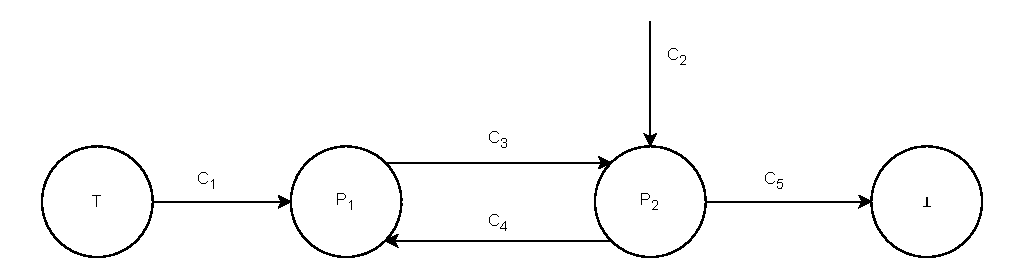
\includegraphics[width=1\textwidth]{Figures/ConciseEx.pdf}
        \caption{Graph representation of CHC System~\ref{fig:chcConc}}
   \end{minipage}
\end{figure}

\end{subfigures}

Consider the CHC system in Figure~\ref{fig:chcConc}. 
This system contains two simple paths from $\top$ to $\bot$: $\proute_1 = [\clause_1, \clause_3, 
\clause_5]$ and $\proute_2 = [\clause_2, \clause_5]$. 
A concise expansion of $\proute_1$ over $\pred_1$ with respect to the prefix simple path
$\proute_{\pred_1}^\top = [\clause_1]$ would look like: $\cexp(\proute_1, \{\pred_1\}) = [\clause_1]  
\oplus \route_{\pred_1}^{\pred_1} \oplus [\clause_3, \clause_5]$
Here, $\route_{\pred_1}^{\pred_1}$ consists of one or more iterations of the cycle $[\clause_3, \clause_4]$.
However, for $\proute_1$, a concise expansion over predicate $\pred_2$ does not exist. 
This is because cycles over $\pred_2$ are formed by $\iteration_{\pred_2}^{\pred_2} = 
[\clause_4, \clause_3]$, but $\predsf([\clause_4, \clause_3]) \cap \predsf([\clause_1, \clause_3]) = 
\{\pred_1, \pred_2\}$. 
This violates the conciseness condition.
In contrast, a concise expansion of $\proute_2$ over $\pred_2$ does exist, since 
$\predsf(\route_{\pred_2}^{\pred_2}) \cap \predsf([\clause_2]) = \{\pred_2\}$. 
Therefore, $\cexp(\proute_2, \{\pred_2\}) = [\clause_2] \oplus \route_{\pred_2}^{\pred_2} \oplus 
[\clause_5]$ is a concise expansion.
\end{example}

It possible to prove that any possible path through the CHC system is a simple path or concise expansion of a 
simple path.

\begin{lemma}[Concise predicate expansions]\label{Lem:concise}
    Given a CHC system $\system$ over predicates $\preds$, $\sourcepred, \targetpred \in \preds$, any
    path $\route_{\targetpred}^{\sourcepred}$ is either a simple path 
    $\proute_{\targetpred}^{\sourcepred}$, or a concise expansion of a simple path 
    $\route_{\targetpred}^{\sourcepred} = \cexp(\proute_{\targetpred}^{\sourcepred}, [\dots])$.
\end{lemma}

\begin{proof}
    We prove this lemma by induction on the length of the path $\route_{\targetpred}^{\sourcepred}$.

    %

    \textbf{Base case}: If $|\route_{\targetpred}^{\sourcepred}| = 1$, then the path consists of a 
    single clause $\clause^{\sourcepred}_{\targetpred}$. By definition, this is a simple path.

    %

    \textbf{Inductive case}: Assume the lemma holds for all paths of length $n$. Consider a path of 
    length $n+1$ formed by appending a clause $\clause_{\pred}^{\targetpred}$ to an existing 
    path $\route^\sourcepred_\targetpred$ of length $n$.  It is sufficient to only consider adding a 
    clause to the end of $\route^\sourcepred_\targetpred$.

    %

    Let us consider a path of size $n$:
        $[\clause_1, \dots, \clause_{n-1}, \clause_n]$. 
    If clause $\clause$ is added in the beginning (or in the middle) of it, we get a new path:
        $[\clause, \clause_1, \dots, \clause_{n-1}, \clause_n]$. 
    By our inductive assumption all paths of size $n$ are either concise expansions of simple 
    paths or simple paths, then $[\clause, \clause_1, \dots, \clause_{n-1}]$ is a concise 
    expansion or a simple path. 
    Therefore it is the same problem as adding $\clause_n$ to simple path or concise expansion 
    $[\clause, \clause_1, \dots, \clause_{n-1}]$, and it is sufficient to consider only the case
    when $\clause$ is added to the end of the path.

    %

    We consider two cases, depending on whether the initial path $\route^\sourcepred_\targetpred$ 
    is a simple path or a concise expansion of a simple path.

    %

    \textbf{Case 1}: Let us consider appending a clause $\clause_{\pred}^{\targetpred}$ to the simple path
    $\proute_{\targetpred}^{\sourcepred}$. 
    There are two sub-cases:
    \begin{itemize}
        \item If $\forall \clause \in \proute_{\targetpred}^{\sourcepred}$: $\source(\clause) \neq 
            \targetpred$ and $\target(\clause) \neq \pred$, then the extended path remains a simple 
            path: $\proute^\sourcepred_\pred = \proute^\sourcepred_\targetpred \oplus 
            [\clause^\targetpred_\pred]$.
        \item Otherwise, appending $\clause$ would introduce a cycle. There are two possibilities:
        \begin{itemize}
            \item $\exists \clause \in \proute_{\targetpred}^{\sourcepred}$ such that 
                $\source(\clause) = \targetpred$. This can happen only if $\sourcepred = \targetpred$. 
                Otherwise, path would contain clauses $\clause_\targetpred^*, \clause^\targetpred_*$ 
                and the last clause is also $\clause_\targetpred^*$, which contradicts definition of a
                simple path (since there would exist multiple clauses in $\proute^\sourcepred_\targetpred$
                such that $\target(\clause) = \targetpred$). 
                In this case, the extended path becomes 
                $\proute_{\targetpred}^{\targetpred} \oplus [\clause^{\targetpred}_{\pred}]$, which 
                is a concise expansion: $\cexp([\clause^{\targetpred}_{\pred}], \{\targetpred\})$.  
            \item $\exists \clause \in \proute_{\targetpred}^{\sourcepred}$ such that 
                $\target(\clause) = \pred$. Then, the simple path can be written as 
                $\proute_{\targetpred}^{\sourcepred} = \proute_{\pred}^{\sourcepred} \oplus 
                \proute_{\targetpred}^{\pred}$, and the extended path becomes  $\proute^\sourcepred_\pred 
                \oplus \proute^\pred_\targetpred \oplus [\clause^\targetpred_\pred]$, where 
                $\proute_{\targetpred}^{\pred} \oplus [\clause_{\pred}^{\targetpred}] = 
                \route_{\pred}^{\pred}$ forms a cycle. Since $\predsf(\route_{\pred}^{\pred}) \cap
                \predsf(\proute_{\pred}^{\sourcepred}) = \{\pred\}$, the new path is a concise 
                expansion: $\cexp(\proute_{\pred}^{\sourcepred}, \{\pred\})$.
        \end{itemize}
    \end{itemize}

%

    \textbf{Case 2}: Let us consider appending $\clause_{\pred}^{\targetpred}$ to a concise
    expansion $\route_{\targetpred}^{\sourcepred} = \cexp(\proute_{\targetpred}^{\sourcepred}, \{\dots\})$.
    This means the path can be written as:
    \[
        \route_{\targetpred}^{\sourcepred} = \route_{\sourcepred}^{\sourcepred} \oplus 
        [\clause^{\sourcepred}_{*}] \oplus \dots \oplus [\clause^{*}_{\targetpred}] \oplus 
        \route_{\targetpred}^{\targetpred}
    \]
    where each cycle $\route_{\sourcepred}^{\sourcepred}, \dots,\route_{\targetpred}^{\targetpred}$ is
    concise with respect to the corresponding simple prefix $\emptyset, \dots, 
    \proute_{\targetpred}^{\sourcepred} \subseteq \proute_{\targetpred}^{\sourcepred}$.

    \begin{itemize}
        \item If $\forall \clause \in \proute_{\targetpred}^{\sourcepred}$: 
            $\source(\clause) \neq \targetpred$ and $\target(\clause) \neq \pred$, then the 
            resulting path remains a concise expansion $\cexp(\proute_{\pred}^{\sourcepred}, \{\dots\})$
            of a longer simple path $\proute_{\pred}^{\sourcepred} = \proute_{\targetpred}^{\sourcepred}
            \oplus [\clause_{\pred}^{\targetpred}]$ over same predicates.
        \item Otherwise, as in the simple path case, two situations may occur:
        \begin{itemize}
            \item $\exists \clause \in \proute_{\targetpred}^{\sourcepred}$ such that 
                $\source(\clause) = \targetpred$. This again implies $\sourcepred = \targetpred$, 
                and the path can be rewritten as $\cexp([\clause^{\targetpred}_{\pred}], \{\targetpred\})$.
            \item$\exists \clause \in \proute_{\targetpred}^{\sourcepred}$ such that 
                $\target(\clause) = \pred$. The original path can be rewritten as:
                \[
                    \route_{\targetpred}^{\sourcepred} = \route^\sourcepred_\sourcepred \oplus 
                    [\clause^\sourcepred_*] \oplus \dots \oplus [\clause^*_\pred] \oplus 
                    \route_\pred^\pred \oplus  [\clause_*^\pred]\oplus \dots \oplus 
                    [\clause^*_\targetpred] \oplus \route^\targetpred_\targetpred
                \]
                When clause $\clause_\pred^\targetpred$ is added to $\route_{\targetpred}^{\sourcepred}$,
                then $(\route_\pred^\pred \oplus  [\clause_*^\pred]\oplus \dots 
                \oplus [\clause^*_\targetpred] \oplus \route^\targetpred_\targetpred) 
                \oplus \clause_\pred^\targetpred$ forms a cycle $\route_\pred^\pred$, 
                and overall path can be rewritten as follows:
                \[
                \route_{\targetpred}^{\sourcepred} = \route_{\sourcepred}^{\sourcepred} \oplus 
                    [\clause^{\sourcepred}_{*}] \oplus \dots \oplus [\clause^{*}_{\pred}] \oplus 
                    \route_{\pred}^{\pred}
                \]
            where $\predsf(\route_{\pred}^{\pred}) \cap \predsf(\proute_{\pred}^{\sourcepred}) = 
            \{\pred\}$. Therefore the resulting path is a concise expansion: 
            $\cexp(\proute_{\pred}^{\sourcepred}, \{\dots, \pred\})$ where 
            $\proute_{\pred}^{\sourcepred} \subseteq \proute_{\targetpred}^{\sourcepred}$ is simple prefix.

        \end{itemize}
        
    \end{itemize}
    
    By structural induction, we have shown that any path is either a simple path or a concise 
    expansion of a simple path.
\end{proof}

\begin{lemma}[Iteration Overapproximation]\label{Lem:mu}
    Let \emph{\mergeTransition} called over a CHC system $\system$, a set of blocked predicates $\preds_b$,
    a map of summaries $\summaries$, 
    and a predicate $\pred$, return a formula $\mu$. 
    Then, for any iteration path $\iteration_\pred^\pred$ such that $\iteration_\pred^\pred \cap 
    \preds_b = \emptyset$:
    $\encoding(\iteration_\pred^\pred)(x^{(0)}, \dots, x^{(n)}) \implies \mu(x^{(0)}, \dots, x^{(n)}).$
\end{lemma}

\begin{proof}
    Let us prove this lemma by contradiction. Assume there exists an iteration path 
    $\iteration^\pred_\pred$ such that $\iteration^\pred_\pred \cap \preds_b 
    = \emptyset$ and $\encoding(\iteration^\pred_\pred)(x^{(0)}, \dots, x^{(n)}) \land \lnot 
    \mu(x^{(0)}, \dots, x^{(n)})$ is satisfiable. 

    By Lemma~\ref{Lem:concise}, any path $\iteration^\pred_\pred$ is either 
    a simple path $\proute_\pred^\pred$, or a concise expansion of a simple path
    $\proute_\pred^\pred = [\clause_1, \dots, \clause_m]$. 
    Therefore, the iteration can be written as $\iteration_\pred^\pred = \cexp(\proute_\pred^\pred, 
    \dots)$ = $[\clause_1] \oplus \route^{\source(\clause_2)}_{\source(\clause_2)} \oplus [\clause_2] 
    \oplus \dots  \oplus \route^{\source(\clause_m)}_{\source(\clause_m)} \oplus \clause_m$ 
    where each cycle path $\route^{\source(\clause)}_{\source(\clause)}$ for 
    $\clause \in \proute_\pred^\pred$ is either an empty path or a concise
    cycle path with respect to $\predsf(\proute^\pred_{\source(\clause)}) \setminus \source(\clause)$. 
    Importantly, there are no cycle paths $\route^{\pred}_{\pred}$ present in $\iteration^\pred_\pred$
    ($\route^{\source(\clause_1)}_{\source(\clause_1)}$ and 
    $\route^{\target(\clause_m)}_{\target(\clause_m)}$), since otherwise 
    $\iteration^\pred_\pred$ would not be an iteration path.
    If for every clause $\clause \in \proute_\pred^\pred$ corresponding cycle path 
    $\route^{\source(\clause)}_{\source(\clause)}$ in $\iteration_\pred^\pred$ is empty, then 
    $\iteration_\pred^\pred$ is a simple path.
    
    As described in Subsection~\ref{Section:Summarize}, $\mu = \bigvee \mu_{\proute}$, where each 
    $\mu_{\proute}$ corresponds to a specific simple path $\proute_\pred^\pred$. 
    By our initial assumption, $\encoding(\iteration^\pred_\pred) \land \lnot \mu$ is satisfiable,
    so $\encoding(\iteration^\pred_\pred) \land \lnot \mu_{\proute}$
    is also satisfiable for every $\mu_{\proute}$.
    Let us consider specifically $\mu_{\proute}$, which was constructed for the same simple path as used 
    in the considered iteration $\iteration^\pred_\pred = \cexp(\proute_\pred^\pred, \dots)$. 
    The conjunction $\encoding(\iteration^\pred_\pred) \land \lnot \mu_{\proute}$ can be 
    written as:
    {\footnotesize
    \begin{align*}
        \encoding(\iteration^\pred_\pred)&(x^{(0)}, \dots, x^{(n)}) \land \lnot 
            \mu_{\proute}(x^{(0)}, \dots, x^{(n)}) = \\
        ( \\
        & \constraint(\clause_1)(x^{(0)}, x^{(1)})\ \land  && (\clause_1) \\ 
        & \big(\encoding(\route_{\source(\clause_2)}^{\source(\clause_2)})(x^{(1)}, \dots, x^{(i)}) 
            \land \constraint(\clause_2)(x^{(i)}, x^{(i+1)})\big)\ \land   && (\clause_2) \\ 
        & \dots\ \land \\ 
        & \big(\encoding(\route_{\source(\clause_m)}^{\source(\clause_m)})(x^{(j)}, \dots, x^{(n-1)})
            \land \constraint(\clause_m)(x^{(n-1)}, x^{(n)})\big)  && (\clause_m) \\
        ) \land \lnot ( \\
        &  \constraint(\clause_1)(x^{(0)}, x^{(1)}) \land  && (\clause_1)\\
        & \big(\constraint(\clause_2)(x^{(1)}, x^{(i+1)}) \lor 
            (\summaries(\source(\clause_2), \preds_b)(x^{(1)}, x^{(i)}) \land 
            \constraint(\clause_2)(x^{(i)}, x^{(i+1)}))\big)\ \land  && (\clause_2)\\
        & \dots\ \land \\
        & \big(\constraint(\clause_m)(x^{(j)}, x^{(n)}) \lor  
            (\summaries(\source(\clause_m),  (\predsf(\proute) \setminus \{\source(\clause_m)\}) \cup 
            \preds_b)(x^{(j)}, x^{(n-1)}) && (\clause_m)\\ 
        &   \land \constraint(\clause_m)(x^{(n-1)}, x^{(n)})) \big)  \\
        ).
    \end{align*}
    }
    The formula $\encoding(\iteration^\pred_\pred)(x^{(0)}, \dots, x^{(n)}) \land \lnot 
    \mu_{\proute}(x^{(0)}, \dots, x^{(n)})$ is unsatisfiable. To prove it, let us show that 
    $\encoding(\iteration^\pred_\pred)(x^{(0)}, \dots, x^{(n)})$ is UNSAT when conjoined with negation
    of any conjunct in $\mu_{\proute}$. 
    
    As demonstrated above, every conjunct in 
    $\encoding(\iteration^\pred_\pred)$ and in $\mu_{\proute}$ can be mapped to the specific clause 
    $\clause_i \in \proute^\sourcepred_\targetpred$ (in the column on the right). 
    By conjoining conjuncts in $\encoding(\iteration^\pred_\pred)$ with the negations of corresponding
    conjuncts in $\mu_{\proute}$ is is possible to demonstrate that $\encoding(\iteration^\pred_\pred)(x^{(0)}, 
    \dots, x^{(n)}) \land \lnot \mu_{\proute}(x^{(0)}, \dots, x^{(n)})$ is unsatisfiable.

    First, consider the case of $\encoding(\iteration^\pred_\pred)(x^{(0)}, \dots, x^{(n)}) \land 
    \lnot \constraint(\clause_1)(x^{(0)}, x^{(1)})$. This is trivially unsatisfiable since 
    $\constraint(\clause_1)(x^{(0)}, x^{(1)})$ is a conjunct in $\encoding(\iteration^\pred_\pred)$.

    Now, consider any conjunct $conj_\mu$ in $\mu_\proute$ mapped to 
    some clause $\clause_i \in \proute_\pred^\pred$, with $\source(\clause_i) = q$:
    $$conj_\mu(x^{(k)}, x^{(l)}, x^{(l+1)}) = (\summaries(q, \preds_b')(x^{(k)}, x^{(l)}) \land
    \constraint(\clause_i)(x^{(l)}, x^{(l+1)})) \lor \constraint(\clause_i)(x^{(k)}, x^{(l+1)}).$$    
    where $\preds_b'= \preds_b \cup \{\pred\} \cup (\predsf(\proute^\pred_{\source(\clause_i)}) \setminus \{\source(\clause_i)\})$ 
    and $\proute^\pred_{\source(\clause_i)} \subseteq \proute^\pred_\pred$.
    The corresponding conjunct $conj_{\iteration}$ in $\encoding(\iteration^\pred_\pred)$ is:
    $$conj_{\iteration}(x^{(k)}, \dots, x^{(l+1)}) =  (\encoding(\route_{q}^{q})(x^{(k)}, \dots, x^{(l)})
    \land \constraint(\clause_i)(x^{(l)}, x^{(l+1)})).$$
    And overall formula:
    \begin{align*}
        &conj_\iteration(x^{(k)}, \dots, x^{(l+1)}) \land \lnot conj_\mu(x^{(k)}, x^{(l)}, x^{(l+1)}) = \\ 
        &\big(conj_\iteration(x^{(k)}, \dots, x^{(l+1)}) \land 
            \lnot (\summaries(q, \preds_b')(x^{(k)}, x^{(l)}) \land 
            \constraint(\clause_i)(x^{(l)}, x^{(l+1)}))\big) \land \\
        &\big(conj_\iteration(x^{(k)}, \dots, x^{(l+1)}) \land 
            \lnot  \constraint(\clause_i)(x^{(k)}, x^{(l+1)})\big).
    \end{align*}
    % conj_\iteration \land \lnot conj_\mu = $$
    There are two cases for $conj_\iteration$. First, when $\route_{q}^{q} = \emptyset$, then
    $k = l$ and:
    $$conj_\iteration(x^{(k)}, x^{(l+1)}) = \constraint(\clause_i)(x^{(k)}, x^{(l+1)})$$
    Since $\constraint(\clause_i)(x^{(k)}, x^{(l+1)}) \land \lnot
    \constraint(\clause_i)(x^{(k)}, x^{(l+1)})$ is unsatisfiable, $conj_\iteration \land \lnot conj_\mu$ is 
    also unsatisfiable.

    %

    Otherwise, if $\route_{q}^{q} \neq \emptyset$, then by the definition of summary,
    $\encoding(\route_{q}^{q})(x^{(k)}, \dots, x^{(l)}) \land \lnot \summaries(q, \preds_b')(x^{(k)}, x^{(l)})$ 
    is unsatisfiable since $\route_{q}^{q}$ is concise with respect to $\preds_b'$. 
    Therefore, 
    \begin{align*}
    & \big((\encoding(\route_{q}^{q})(x^{(k)}, \dots, x^{(l)}) \land 
    \constraint(\clause_i)(x^{(l)}, x^{(l+1)})) \land \lnot \summaries(q, \preds_b')(x^{(k)}, x^{(l)}) \big)\ \lor \\
    & \big( (\encoding(\route_{q}^{q})(x^{(k)}, \dots, x^{(l)})
    \land \constraint(\clause_i)(x^{(l)}, x^{(l+1)})) \land \lnot \constraint(\clause_i)(x^{(l)}, x^{(l+1)})\big)
    \end{align*}
    $$$$
    is also unsatisfiable which means that $conj_\iteration \land \lnot conj_\mu$ is unsatisfiable.
    We've demonstrated that for every negation of conjunct $conj_\mu$ in $\mu_{\proute}$, the 
    conjunction $\encoding(\iteration^\pred_\pred) \land \lnot conj_\mu$ is unsatisfiable. 
    Which means that $\encoding(\iteration^\pred_\pred) \land \lnot \mu_{\proute}$ is unsatisfiable.
    It is a contradiction of initial assumption that $\encoding(\iteration^\pred_\pred) 
    \land \lnot \mu$ is satisfiable. This completes the proof.
\end{proof}

\begin{lemma}[Cycle summarization]\label{Lem:expSat}
    If \emph{\summarize}, invoked over CHC System $\system$ with a set of blocked predicates $\preds_b$ 
    and Pre/Post formulas $\precond, \postcond$, returns a tuple 
    $\tuple{\emptyset, \summaries}$, then no feasible cycle 
    path $\route_{\pred}^{\pred}$ with $\predsf(\route_{\pred}^{\pred}) \cap \preds_b = \emptyset$ exists, such 
    that $\precond(\dots, x) \land \encoding(\route_{\pred}^{\pred})(x, \dots, x') \land 
    \postcond(x')$ is satisfiable.
\end{lemma}

\begin{proof}
    We prove this lemma by contradiction. 
    Suppose there exists a cycle path 
    $\route_\pred^\pred$ with predicates $\predsf(\route_\pred^\pred) \cap \preds_b = \emptyset$ such 
    that $\precond(\dots, x) \land \encoding(\route_{\pred}^{\pred})(x, \dots, x') \land 
    \postcond(x')$ is satisfiable. 

    Any possible cycle path can be decomposed into multiple iteration paths $\iteration^\pred_\pred$: 
    $\route_\pred^\pred = \iteration_1 \oplus \dots \oplus \iteration_n$. 
    Therefore the path condition can be written as 
    $\encoding(\route_\pred^\pred)(x, \dots, x') = \encoding(\iteration_1)(x, \dots, x^{(i)}) \land \dots 
    \land \encoding(\iteration_n)(x^{(j)}, \dots, x')$. 
    
    \summarize, at Line~\ref{summarize:mtr}, constructs formula $\mu$ to overapproximate 
    all possible iteration paths.
    By construction (Lemma~\ref{Lem:mu}), for any iteration path $\iteration$ with $\predsf(\iteration)
    \cap \preds_b = \emptyset$, it holds that $\encoding(\iteration)(x, \dots, x') \implies 
    \mu(x, \dots, x')$.  
    Thus, $\encoding(\iteration_1)(x, \dots, x^{(i)}) \land \dots \land 
    \encoding(\iteration_n)(x^{(j)}, \dots, x') \implies \mu(x, \dots, x^{(i)}) 
    \land \dots \land \mu(x^{(j)}, \dots, x')$, where each $\encoding(\iteration_i)$ is mapped to 
    a corresponding $\mu$.
    It means that $\precond(\dots, x) \land  \mu(x, \dots, x^{(i)}) 
    \land \dots \land \mu(x^{(j)}, \dots, x') \land \postcond(x')$ is also satisfiable.

    Additionally, by the definition of \tpa which returned $\tuple{\emptyset, \summary_\pred}$, 
    $\mu(x, \dots, x^{(i)}) \land \dots \land \mu(x^{(j)}, \dots, x') \implies \summary_\pred(x,x')$.
    Thus, $\precond(\dots, x) \land \summary_\pred(x, x') \land \postcond(x')$ is
    satisfiable.
    However, by same definition of \tpa $\precond(\dots, x) \land \summary_\pred(x, x') 
    \land \postcond(x')$ is unsatisfiable. 
    This is a contradiction. 
    Therefore, a path $\route_\pred^\pred$ does not exist.
\end{proof}

\begin{lemma}[Pre and Post formulas]~\label{Lem:encodings}
    \emph{\queryUnrolling} \textbf{invariant:}
    Suppose \emph{\queryUnrolling} is called over CHC system $\system$ with blocked predicates 
    $\preds_b$, map of cycle summaries $\summaries$, and Pre, Post formulas 
    $\precond, \postcond$  over a simple path $\proute_\bot^\top$ . 
    For any $\clause_i \in \predsf(\proute_\bot^\top)$, $\source(\clause_i) = \pred$
    there does not exist a feasible concise expansion $\cexp(\proute_\bot^\top, \{\dots, \pred, \dots\}) = 
    \route^{\top}_{\pred} \oplus \route^{\pred}_{\pred} \oplus \route^{\pred}_{\bot}$ 
    such that either of the following formulas is satisfiable: 
    \begin{align*}
        &\encoding(\route^{\top}_{\pred})(x,\dots,x') \land 
            \lnot \precond(\clause_{i})(x') \land \encoding(\route^{\pred}_{\pred} \oplus 
            \route^{\pred}_{\bot})(x', \dots, x'') \\
        &\encoding(\route^{\top}_{\pred} \oplus 
            \route^{\pred}_{\pred})(x,\dots,x') \land \lnot \postcond(\clause_{i})(x') \land 
            \encoding(\route^{\pred}_{\bot})(x',\dots,x'') 
    \end{align*}
\end{lemma}

\begin{proof}
    We prove this lemma by induction. 
    
    \textbf{Base case:} Initially, for all $\clause_i \in \proute_\bot^\top$, 
    both $\precond(\clause_{i})$ and $\postcond(\clause_{i})$  are set to $\top$, so the invariant holds 
    trivially.

    %

    \textbf{Inductive case:} Assume the invariant holds at some point during the execution.
    Pre and Post formulas $\precond(\clause_{i}),\postcond(\clause_{i})$ may be updated at 
    Lines~\ref{queryUnrolling:postcondupd}, \ref{queryUnrolling:precondF}, and 
    \ref{queryUnrolling:precondupd} of Algorithm~\ref{Alg:QueryUnrolling}. 


    %

    On Line~\ref{queryUnrolling:postcondupd}, the algorithm updates $\postcond(\clause_{i})$ when 
    extending the path with a clause from the original simple path $\clause_i \in \proute^{\top}_{\bot}$, 
    $\source(\clause_i) = \pred$.
    The update at Line~\ref{queryUnrolling:postcondupd} 
    maintains following relation by construction: $\lnot \postcond(\clause_i)(x) 
    \land \constraint(\clause_i)(x,x') \implies \lnot \precond(\clause_{i+1})(x')$. 
    Since for $\lnot \precond(\clause_{i+1})$ invariant holds, then it also holds for 
    $\postcond(\clause_i)$.

    %

    On Line~\ref{queryUnrolling:precondF}, the precondition $\precond(\clause_i)$ is strengthened based 
    on the cycle summary $\summaries(\pred, \preds_b)$. For any concise cycle path $\route^i_i$
    following formula $\lnot \precond(\clause_i)(x) \land \route^i_i(x,x') \land 
    \postcond(\clause_i)(x')$ is UNSAT (based on the definition of cycle summary).
    Therefore,  $\lnot \precond(\clause_i)(x) \land \summaries(\pred, \preds_b)(x,x') \implies \lnot 
    \postcond(\clause_i)(x')$. 
    Since $\encoding(\route^{\sourcepred}_{\pred} \oplus 
            \route^{\pred}_{\pred})(x,\dots,x') \land \lnot \postcond(\clause_i)(x') \land 
            \encoding(\route^{\pred}_{\targetpred})(x',\dots,x'')$ is unsatisfiable,
    invariant still holds for $\precond(\clause_i)$.
    % Since $\encoding(\route^{\sourcepred}_{\pred} \oplus 
    %         \route^{\pred}_{\pred})(x,\dots,x') \land \lnot \postcond_i(x') \land 
    %         \encoding(\route^{\pred}_{\targetpred})(x',\dots,x'')$ is 
    % unsatisfiable, and for new $\precond_\pred$ it holds that  $\lnot \precond_\pred(x) \land 
    % \summaries(\pred, \preds_b)(x,x') \implies \lnot \postcond_\pred(x')$, thus, 
    % $\encoding(\route^{\sourcepred}_{\pred})(x,\dots,x') \land 
    %         \lnot \precond_{i}(x') \land \encoding(\route^{\pred}_{\pred} \oplus 
    %         \route^{\pred}_{\targetpred})(x', \dots, x'') $ is also unsatisfiable.
    
    %

    Finally, on Line~\ref{queryUnrolling:precondupd} Pre formula $\precond(\clause_i)$ is updated as
    $\precond(\clause_i) \gets \postcond(\clause_i)$, which preserves the invariant since concise cycle 
    over $\pred$ does not exist.
    Therefore, in all cases, the updates to $\precond(\clause_i)$ and $\postcond(\clause_i)$ preserve the 
    invariant.
\end{proof}


The proof for \textbf{Theorem}~\ref{Thm:SAT} is given below.

\begin{proof}
    The proof follows from Lemma~\ref{Lem:encodings} and Lemma~\ref{Lem:concise}. 
    Algorithm~\ref{Alg:solveCHC} invokes \queryUnrolling to determine whether any simple 
    path $\proute^\top_\bot$ in the CHC system can be expanded into a satisfiable path. 
    \queryUnrolling returns $\emptyset$ only when it enters "if" at 
    Line~\ref{queryUnrolling:noRouteCheck}, which means $\constraint(\clause_1) \land 
    \precond(\clause_{2})$ is unsatisfiable.
    By Lemma~\ref{Lem:encodings}, it means that there does not exist a feasible concise expansion 
    $\cexp(\proute^{\top}_{\bot}, \dots)$, since $\constraint(\clause_1) \land \precond((\clause_{2})) 
    \land \route^{\source(\clause_2)}_\targetpred$ is unsatisfiable for any concise 
    $\route^{\source(\clause_2)}_\targetpred$.
    \solveCHC calls \queryUnrolling for every simple path $\proute_{\bot}^{\top}$ in the CHC system,
    and only if none of these paths can be expanded into a satisfiable path it returns \textsc{SAFE}.

    From Lemma~\ref{Lem:concise}, any path through the CHC system is either a simple path 
    or a \emph{concise} expansion of a simple path. 
    Hence, if Algorithm~\ref{Alg:solveCHC} returns \textsc{SAFE}, there does not exist a feasible path 
    $\route_\bot^\top$ through the system.
\end{proof}


\end{document}
